% Options for packages loaded elsewhere
\PassOptionsToPackage{unicode}{hyperref}
\PassOptionsToPackage{hyphens}{url}
%
\documentclass[
]{article}
\usepackage{amsmath,amssymb}
\usepackage{iftex}
\ifPDFTeX
  \usepackage[T1]{fontenc}
  \usepackage[utf8]{inputenc}
  \usepackage{textcomp} % provide euro and other symbols
\else % if luatex or xetex
  \usepackage{unicode-math} % this also loads fontspec
  \defaultfontfeatures{Scale=MatchLowercase}
  \defaultfontfeatures[\rmfamily]{Ligatures=TeX,Scale=1}
\fi
\usepackage{lmodern}
\ifPDFTeX\else
  % xetex/luatex font selection
\fi
% Use upquote if available, for straight quotes in verbatim environments
\IfFileExists{upquote.sty}{\usepackage{upquote}}{}
\IfFileExists{microtype.sty}{% use microtype if available
  \usepackage[]{microtype}
  \UseMicrotypeSet[protrusion]{basicmath} % disable protrusion for tt fonts
}{}
\makeatletter
\@ifundefined{KOMAClassName}{% if non-KOMA class
  \IfFileExists{parskip.sty}{%
    \usepackage{parskip}
  }{% else
    \setlength{\parindent}{0pt}
    \setlength{\parskip}{6pt plus 2pt minus 1pt}}
}{% if KOMA class
  \KOMAoptions{parskip=half}}
\makeatother
\usepackage{xcolor}
\usepackage[top=25mm,left=25mm,margin=1in]{geometry}
\usepackage{color}
\usepackage{fancyvrb}
\newcommand{\VerbBar}{|}
\newcommand{\VERB}{\Verb[commandchars=\\\{\}]}
\DefineVerbatimEnvironment{Highlighting}{Verbatim}{commandchars=\\\{\}}
% Add ',fontsize=\small' for more characters per line
\usepackage{framed}
\definecolor{shadecolor}{RGB}{248,248,248}
\newenvironment{Shaded}{\begin{snugshade}}{\end{snugshade}}
\newcommand{\AlertTok}[1]{\textcolor[rgb]{0.94,0.16,0.16}{#1}}
\newcommand{\AnnotationTok}[1]{\textcolor[rgb]{0.56,0.35,0.01}{\textbf{\textit{#1}}}}
\newcommand{\AttributeTok}[1]{\textcolor[rgb]{0.13,0.29,0.53}{#1}}
\newcommand{\BaseNTok}[1]{\textcolor[rgb]{0.00,0.00,0.81}{#1}}
\newcommand{\BuiltInTok}[1]{#1}
\newcommand{\CharTok}[1]{\textcolor[rgb]{0.31,0.60,0.02}{#1}}
\newcommand{\CommentTok}[1]{\textcolor[rgb]{0.56,0.35,0.01}{\textit{#1}}}
\newcommand{\CommentVarTok}[1]{\textcolor[rgb]{0.56,0.35,0.01}{\textbf{\textit{#1}}}}
\newcommand{\ConstantTok}[1]{\textcolor[rgb]{0.56,0.35,0.01}{#1}}
\newcommand{\ControlFlowTok}[1]{\textcolor[rgb]{0.13,0.29,0.53}{\textbf{#1}}}
\newcommand{\DataTypeTok}[1]{\textcolor[rgb]{0.13,0.29,0.53}{#1}}
\newcommand{\DecValTok}[1]{\textcolor[rgb]{0.00,0.00,0.81}{#1}}
\newcommand{\DocumentationTok}[1]{\textcolor[rgb]{0.56,0.35,0.01}{\textbf{\textit{#1}}}}
\newcommand{\ErrorTok}[1]{\textcolor[rgb]{0.64,0.00,0.00}{\textbf{#1}}}
\newcommand{\ExtensionTok}[1]{#1}
\newcommand{\FloatTok}[1]{\textcolor[rgb]{0.00,0.00,0.81}{#1}}
\newcommand{\FunctionTok}[1]{\textcolor[rgb]{0.13,0.29,0.53}{\textbf{#1}}}
\newcommand{\ImportTok}[1]{#1}
\newcommand{\InformationTok}[1]{\textcolor[rgb]{0.56,0.35,0.01}{\textbf{\textit{#1}}}}
\newcommand{\KeywordTok}[1]{\textcolor[rgb]{0.13,0.29,0.53}{\textbf{#1}}}
\newcommand{\NormalTok}[1]{#1}
\newcommand{\OperatorTok}[1]{\textcolor[rgb]{0.81,0.36,0.00}{\textbf{#1}}}
\newcommand{\OtherTok}[1]{\textcolor[rgb]{0.56,0.35,0.01}{#1}}
\newcommand{\PreprocessorTok}[1]{\textcolor[rgb]{0.56,0.35,0.01}{\textit{#1}}}
\newcommand{\RegionMarkerTok}[1]{#1}
\newcommand{\SpecialCharTok}[1]{\textcolor[rgb]{0.81,0.36,0.00}{\textbf{#1}}}
\newcommand{\SpecialStringTok}[1]{\textcolor[rgb]{0.31,0.60,0.02}{#1}}
\newcommand{\StringTok}[1]{\textcolor[rgb]{0.31,0.60,0.02}{#1}}
\newcommand{\VariableTok}[1]{\textcolor[rgb]{0.00,0.00,0.00}{#1}}
\newcommand{\VerbatimStringTok}[1]{\textcolor[rgb]{0.31,0.60,0.02}{#1}}
\newcommand{\WarningTok}[1]{\textcolor[rgb]{0.56,0.35,0.01}{\textbf{\textit{#1}}}}
\usepackage{graphicx}
\makeatletter
\def\maxwidth{\ifdim\Gin@nat@width>\linewidth\linewidth\else\Gin@nat@width\fi}
\def\maxheight{\ifdim\Gin@nat@height>\textheight\textheight\else\Gin@nat@height\fi}
\makeatother
% Scale images if necessary, so that they will not overflow the page
% margins by default, and it is still possible to overwrite the defaults
% using explicit options in \includegraphics[width, height, ...]{}
\setkeys{Gin}{width=\maxwidth,height=\maxheight,keepaspectratio}
% Set default figure placement to htbp
\makeatletter
\def\fps@figure{htbp}
\makeatother
\setlength{\emergencystretch}{3em} % prevent overfull lines
\providecommand{\tightlist}{%
  \setlength{\itemsep}{0pt}\setlength{\parskip}{0pt}}
\setcounter{secnumdepth}{-\maxdimen} % remove section numbering
\ifLuaTeX
  \usepackage{selnolig}  % disable illegal ligatures
\fi
\usepackage{bookmark}
\IfFileExists{xurl.sty}{\usepackage{xurl}}{} % add URL line breaks if available
\urlstyle{same}
\hypersetup{
  pdftitle={Happiness 2017},
  pdfauthor={Fernando Huilca},
  hidelinks,
  pdfcreator={LaTeX via pandoc}}

\title{Happiness 2017}
\usepackage{etoolbox}
\makeatletter
\providecommand{\subtitle}[1]{% add subtitle to \maketitle
  \apptocmd{\@title}{\par {\large #1 \par}}{}{}
}
\makeatother
\subtitle{Original Author: Javad Zabihi}
\author{Fernando Huilca}
\date{31/01/2025}

\begin{document}
\maketitle

{
\setcounter{tocdepth}{2}
\tableofcontents
}
\section{Introduction}\label{introduction}

The dataset that we have chosen is happiness 2017 dataset, one of
Kaggle's dataset. This dataset gives the happiness rank and happiness
score of 155 countries around the world based on seven factors including
family, life expectancy, economy, generosity, trust in government,
freedom, and dystopia residual. Sum of the value of these seven factors
gives us the happiness score and the higher the happiness score, the
lower the happiness rank. So, it is evident that the higher value of
each of these seven factors means the level of happiness is higher. We
can define the meaning of these factors as the extent to which these
factors lead to happiness. Dystopia is the opposite of utopia and has
the lowest happiness level. Dystopia will be considered as a reference
for other countries to show how far they are from being the poorest
country regarding happiness level.

There are three parts to my report as follows:

\begin{itemize}
\tightlist
\item
  Cleaning
\item
  Visualization
\item
  Prediction
\end{itemize}

\subsection{Mission}\label{mission}

The purpose of choosing this work is to find out which factors are more
important to live a happier life. As a result, people and countries can
focus on the more significant factors to achieve a higher happiness
level. We also will implement several machine learning algorithms to
predict the happiness score and compare the result to discover which
algorithm works better for this specific dataset.

\section{Cleaning}\label{cleaning}

Now we can load our dataset and see the structure of happiness
variables. Our dataset is pretty clean, and we will implement a few
adjustments to make it looks better.

\begin{Shaded}
\begin{Highlighting}[]
\FunctionTok{library}\NormalTok{(plyr)}
\FunctionTok{library}\NormalTok{(dplyr)}
\FunctionTok{library}\NormalTok{(tidyverse)}
\FunctionTok{library}\NormalTok{(lubridate)}
\FunctionTok{library}\NormalTok{(caTools)}
\FunctionTok{library}\NormalTok{(ggplot2)}
\FunctionTok{library}\NormalTok{(ggthemes)}
\FunctionTok{library}\NormalTok{(reshape2)}
\FunctionTok{library}\NormalTok{(data.table)}
\FunctionTok{library}\NormalTok{(tidyr)}
\FunctionTok{library}\NormalTok{(corrgram)       }
\FunctionTok{library}\NormalTok{(corrplot)}
\FunctionTok{library}\NormalTok{(formattable)}
\FunctionTok{library}\NormalTok{(cowplot)}
\FunctionTok{library}\NormalTok{(ggpubr)}
\FunctionTok{library}\NormalTok{(plot3D)}
\end{Highlighting}
\end{Shaded}

\begin{Shaded}
\begin{Highlighting}[]
\CommentTok{\# World happiness report 2017}
\NormalTok{Happiness }\OtherTok{\textless{}{-}} \FunctionTok{read.csv}\NormalTok{(}\StringTok{"C:}\SpecialCharTok{\textbackslash{}\textbackslash{}}\StringTok{Users}\SpecialCharTok{\textbackslash{}\textbackslash{}}\StringTok{Fernando\_Huilca}\SpecialCharTok{\textbackslash{}\textbackslash{}}\StringTok{Desktop}\SpecialCharTok{\textbackslash{}\textbackslash{}}\StringTok{EPN{-}FernandoHuilca}\SpecialCharTok{\textbackslash{}\textbackslash{}}\StringTok{Cuarto Semestre}\SpecialCharTok{\textbackslash{}\textbackslash{}}\StringTok{Sistemas de la información}\SpecialCharTok{\textbackslash{}\textbackslash{}}\StringTok{Cursos}\SpecialCharTok{\textbackslash{}\textbackslash{}}\StringTok{Practica ML R2}\SpecialCharTok{\textbackslash{}\textbackslash{}}\StringTok{Practica ML R 2}\SpecialCharTok{\textbackslash{}\textbackslash{}}\StringTok{2017.csv"}\NormalTok{)}

\FunctionTok{str}\NormalTok{(Happiness)}
\end{Highlighting}
\end{Shaded}

\begin{verbatim}
## 'data.frame':    155 obs. of  12 variables:
##  $ Country                      : chr  "Norway" "Denmark" "Iceland" "Switzerland" ...
##  $ Happiness.Rank               : int  1 2 3 4 5 6 7 8 9 10 ...
##  $ Happiness.Score              : num  7.54 7.52 7.5 7.49 7.47 ...
##  $ Whisker.high                 : num  7.59 7.58 7.62 7.56 7.53 ...
##  $ Whisker.low                  : num  7.48 7.46 7.39 7.43 7.41 ...
##  $ Economy..GDP.per.Capita.     : num  1.62 1.48 1.48 1.56 1.44 ...
##  $ Family                       : num  1.53 1.55 1.61 1.52 1.54 ...
##  $ Health..Life.Expectancy.     : num  0.797 0.793 0.834 0.858 0.809 ...
##  $ Freedom                      : num  0.635 0.626 0.627 0.62 0.618 ...
##  $ Generosity                   : num  0.362 0.355 0.476 0.291 0.245 ...
##  $ Trust..Government.Corruption.: num  0.316 0.401 0.154 0.367 0.383 ...
##  $ Dystopia.Residual            : num  2.28 2.31 2.32 2.28 2.43 ...
\end{verbatim}

We have observed the variables inside our dataset, their class, and the
first few observations of each. In fact, the dataset has 155
observations and 12 variables. I believe some of the variable names are
not clear enough and I decided to change the name of several of them a
little bit. Also, I will remove whisker low and whisker high variables
from my dataset because these variables give only the lower and upper
confidence interval of happiness score and there is no need to use them
for visualization and prediction.

\begin{Shaded}
\begin{Highlighting}[]
\CommentTok{\# Changing the name of columns}
\FunctionTok{colnames}\NormalTok{ (Happiness) }\OtherTok{\textless{}{-}} \FunctionTok{c}\NormalTok{(}\StringTok{"Country"}\NormalTok{, }\StringTok{"Happiness.Rank"}\NormalTok{, }\StringTok{"Happiness.Score"}\NormalTok{,}
                          \StringTok{"Whisker.High"}\NormalTok{, }\StringTok{"Whisker.Low"}\NormalTok{, }\StringTok{"Economy"}\NormalTok{, }\StringTok{"Family"}\NormalTok{,}
                          \StringTok{"Life.Expectancy"}\NormalTok{, }\StringTok{"Freedom"}\NormalTok{, }\StringTok{"Generosity"}\NormalTok{,}
                          \StringTok{"Trust"}\NormalTok{, }\StringTok{"Dystopia.Residual"}\NormalTok{)}


\CommentTok{\# Country: Name of countries}
\CommentTok{\# Happiness.Rank: Rank of the country based on the Happiness Score}
\CommentTok{\# Happiness.Score: Happiness measurement on a scale of 0 to 10}
\CommentTok{\# Whisker.High: Upper confidence interval of happiness score}
\CommentTok{\# Whisker.Low: Lower confidence interval of happiness score}
\CommentTok{\# Economy: The value of all final goods and services produced within a nation in a given year}
\CommentTok{\# Per capita GDP is a measure of the total output of a country that takes the gross domestic product (GDP) and divides it by the number of people in that country. The per capita GDP is especially useful when comparing one country to another, because it shows the relative performance of the countries.}
\CommentTok{\# Family: Importance of having a family}
\CommentTok{\# Life.Expectancy: Importance of health and amount of time prople expect to live}
\CommentTok{\# Freedom: Importance of freedom in each country}
\CommentTok{\# Generosity: The quality of being kind and generous}
\CommentTok{\# Trust: Perception of corruption in a government}
\CommentTok{\# Dystopia.Residual: Plays as a reference}

\CommentTok{\# Deleting unnecessary columns (Whisker.high and Whisker.low)}

\NormalTok{Happiness }\OtherTok{\textless{}{-}}\NormalTok{ Happiness[, }\SpecialCharTok{{-}}\FunctionTok{c}\NormalTok{(}\DecValTok{4}\NormalTok{,}\DecValTok{5}\NormalTok{)]}
\end{Highlighting}
\end{Shaded}

The next step is adding another column to the dataset which is
continent. I want to work on different continents to discover whether
there are different trends for them regarding which factors play a
significant role in gaining higher happiness score. Asia, Africa, North
America, South America, Europe, and Australia are our six continents in
this dataset. Then I moved the position of the continent column to the
second column because I think with this position arrange, dataset looks
better. Finally, I changed the type of continent variable to factor to
be able to work with it easily for visualization. Now we can see the
final structure of our dataset which consisted of 155 observations and
11 variables. Country and continent are factor variables, Happiness rank
is an integer, and the remaining variables are in numeric type.

\begin{Shaded}
\begin{Highlighting}[]
\CommentTok{\# Creating a new column for continents}

\NormalTok{Happiness}\SpecialCharTok{$}\NormalTok{Continent }\OtherTok{\textless{}{-}} \ConstantTok{NA}

\NormalTok{Happiness}\SpecialCharTok{$}\NormalTok{Continent[}\FunctionTok{which}\NormalTok{(Happiness}\SpecialCharTok{$}\NormalTok{Country }\SpecialCharTok{\%in\%} \FunctionTok{c}\NormalTok{(}\StringTok{"Israel"}\NormalTok{, }\StringTok{"United Arab Emirates"}\NormalTok{, }\StringTok{"Singapore"}\NormalTok{, }\StringTok{"Thailand"}\NormalTok{, }\StringTok{"Taiwan Province of China"}\NormalTok{,}
                                   \StringTok{"Qatar"}\NormalTok{, }\StringTok{"Saudi Arabia"}\NormalTok{, }\StringTok{"Kuwait"}\NormalTok{, }\StringTok{"Bahrain"}\NormalTok{, }\StringTok{"Malaysia"}\NormalTok{, }\StringTok{"Uzbekistan"}\NormalTok{, }\StringTok{"Japan"}\NormalTok{,}
                                   \StringTok{"South Korea"}\NormalTok{, }\StringTok{"Turkmenistan"}\NormalTok{, }\StringTok{"Kazakhstan"}\NormalTok{, }\StringTok{"Turkey"}\NormalTok{, }\StringTok{"Hong Kong S.A.R., China"}\NormalTok{, }\StringTok{"Philippines"}\NormalTok{,}
                                   \StringTok{"Jordan"}\NormalTok{, }\StringTok{"China"}\NormalTok{, }\StringTok{"Pakistan"}\NormalTok{, }\StringTok{"Indonesia"}\NormalTok{, }\StringTok{"Azerbaijan"}\NormalTok{, }\StringTok{"Lebanon"}\NormalTok{, }\StringTok{"Vietnam"}\NormalTok{,}
                                   \StringTok{"Tajikistan"}\NormalTok{, }\StringTok{"Bhutan"}\NormalTok{, }\StringTok{"Kyrgyzstan"}\NormalTok{, }\StringTok{"Nepal"}\NormalTok{, }\StringTok{"Mongolia"}\NormalTok{, }\StringTok{"Palestinian Territories"}\NormalTok{,}
                                   \StringTok{"Iran"}\NormalTok{, }\StringTok{"Bangladesh"}\NormalTok{, }\StringTok{"Myanmar"}\NormalTok{, }\StringTok{"Iraq"}\NormalTok{, }\StringTok{"Sri Lanka"}\NormalTok{, }\StringTok{"Armenia"}\NormalTok{, }\StringTok{"India"}\NormalTok{, }\StringTok{"Georgia"}\NormalTok{,}
                                   \StringTok{"Cambodia"}\NormalTok{, }\StringTok{"Afghanistan"}\NormalTok{, }\StringTok{"Yemen"}\NormalTok{, }\StringTok{"Syria"}\NormalTok{))] }\OtherTok{\textless{}{-}} \StringTok{"Asia"}
\NormalTok{Happiness}\SpecialCharTok{$}\NormalTok{Continent[}\FunctionTok{which}\NormalTok{(Happiness}\SpecialCharTok{$}\NormalTok{Country }\SpecialCharTok{\%in\%} \FunctionTok{c}\NormalTok{(}\StringTok{"Norway"}\NormalTok{, }\StringTok{"Denmark"}\NormalTok{, }\StringTok{"Iceland"}\NormalTok{, }\StringTok{"Switzerland"}\NormalTok{, }\StringTok{"Finland"}\NormalTok{,}
                                   \StringTok{"Netherlands"}\NormalTok{, }\StringTok{"Sweden"}\NormalTok{, }\StringTok{"Austria"}\NormalTok{, }\StringTok{"Ireland"}\NormalTok{, }\StringTok{"Germany"}\NormalTok{,}
                                   \StringTok{"Belgium"}\NormalTok{, }\StringTok{"Luxembourg"}\NormalTok{, }\StringTok{"United Kingdom"}\NormalTok{, }\StringTok{"Czech Republic"}\NormalTok{,}
                                   \StringTok{"Malta"}\NormalTok{, }\StringTok{"France"}\NormalTok{, }\StringTok{"Spain"}\NormalTok{, }\StringTok{"Slovakia"}\NormalTok{, }\StringTok{"Poland"}\NormalTok{, }\StringTok{"Italy"}\NormalTok{,}
                                   \StringTok{"Russia"}\NormalTok{, }\StringTok{"Lithuania"}\NormalTok{, }\StringTok{"Latvia"}\NormalTok{, }\StringTok{"Moldova"}\NormalTok{, }\StringTok{"Romania"}\NormalTok{,}
                                   \StringTok{"Slovenia"}\NormalTok{, }\StringTok{"North Cyprus"}\NormalTok{, }\StringTok{"Cyprus"}\NormalTok{, }\StringTok{"Estonia"}\NormalTok{, }\StringTok{"Belarus"}\NormalTok{,}
                                   \StringTok{"Serbia"}\NormalTok{, }\StringTok{"Hungary"}\NormalTok{, }\StringTok{"Croatia"}\NormalTok{, }\StringTok{"Kosovo"}\NormalTok{, }\StringTok{"Montenegro"}\NormalTok{,}
                                   \StringTok{"Greece"}\NormalTok{, }\StringTok{"Portugal"}\NormalTok{, }\StringTok{"Bosnia and Herzegovina"}\NormalTok{, }\StringTok{"Macedonia"}\NormalTok{,}
                                   \StringTok{"Bulgaria"}\NormalTok{, }\StringTok{"Albania"}\NormalTok{, }\StringTok{"Ukraine"}\NormalTok{))] }\OtherTok{\textless{}{-}} \StringTok{"Europe"}
\NormalTok{Happiness}\SpecialCharTok{$}\NormalTok{Continent[}\FunctionTok{which}\NormalTok{(Happiness}\SpecialCharTok{$}\NormalTok{Country }\SpecialCharTok{\%in\%} \FunctionTok{c}\NormalTok{(}\StringTok{"Canada"}\NormalTok{, }\StringTok{"Costa Rica"}\NormalTok{, }\StringTok{"United States"}\NormalTok{, }\StringTok{"Mexico"}\NormalTok{,  }
                                   \StringTok{"Panama"}\NormalTok{,}\StringTok{"Trinidad and Tobago"}\NormalTok{, }\StringTok{"El Salvador"}\NormalTok{, }\StringTok{"Belize"}\NormalTok{, }\StringTok{"Guatemala"}\NormalTok{,}
                                   \StringTok{"Jamaica"}\NormalTok{, }\StringTok{"Nicaragua"}\NormalTok{, }\StringTok{"Dominican Republic"}\NormalTok{, }\StringTok{"Honduras"}\NormalTok{,}
                                   \StringTok{"Haiti"}\NormalTok{))] }\OtherTok{\textless{}{-}} \StringTok{"North America"}
\NormalTok{Happiness}\SpecialCharTok{$}\NormalTok{Continent[}\FunctionTok{which}\NormalTok{(Happiness}\SpecialCharTok{$}\NormalTok{Country }\SpecialCharTok{\%in\%} \FunctionTok{c}\NormalTok{(}\StringTok{"Chile"}\NormalTok{, }\StringTok{"Brazil"}\NormalTok{, }\StringTok{"Argentina"}\NormalTok{, }\StringTok{"Uruguay"}\NormalTok{,}
                                   \StringTok{"Colombia"}\NormalTok{, }\StringTok{"Ecuador"}\NormalTok{, }\StringTok{"Bolivia"}\NormalTok{, }\StringTok{"Peru"}\NormalTok{,}
                                   \StringTok{"Paraguay"}\NormalTok{, }\StringTok{"Venezuela"}\NormalTok{))] }\OtherTok{\textless{}{-}} \StringTok{"South America"}
\NormalTok{Happiness}\SpecialCharTok{$}\NormalTok{Continent[}\FunctionTok{which}\NormalTok{(Happiness}\SpecialCharTok{$}\NormalTok{Country }\SpecialCharTok{\%in\%} \FunctionTok{c}\NormalTok{(}\StringTok{"New Zealand"}\NormalTok{, }\StringTok{"Australia"}\NormalTok{))] }\OtherTok{\textless{}{-}} \StringTok{"Australia"}
\NormalTok{Happiness}\SpecialCharTok{$}\NormalTok{Continent[}\FunctionTok{which}\NormalTok{(}\FunctionTok{is.na}\NormalTok{(Happiness}\SpecialCharTok{$}\NormalTok{Continent))] }\OtherTok{\textless{}{-}} \StringTok{"Africa"}


\CommentTok{\# Moving the continent column\textquotesingle{}s position in the dataset to the second column}

\NormalTok{Happiness }\OtherTok{\textless{}{-}}\NormalTok{ Happiness }\SpecialCharTok{\%\textgreater{}\%} \FunctionTok{select}\NormalTok{(Country,Continent, }\FunctionTok{everything}\NormalTok{())}

\CommentTok{\# Changing Continent column to factor}

\NormalTok{Happiness}\SpecialCharTok{$}\NormalTok{Continent }\OtherTok{\textless{}{-}} \FunctionTok{as.factor}\NormalTok{(Happiness}\SpecialCharTok{$}\NormalTok{Continent)}

\FunctionTok{str}\NormalTok{(Happiness)}
\end{Highlighting}
\end{Shaded}

\begin{verbatim}
## 'data.frame':    155 obs. of  11 variables:
##  $ Country          : chr  "Norway" "Denmark" "Iceland" "Switzerland" ...
##  $ Continent        : Factor w/ 6 levels "Africa","Asia",..: 4 4 4 4 4 4 5 3 4 3 ...
##  $ Happiness.Rank   : int  1 2 3 4 5 6 7 8 9 10 ...
##  $ Happiness.Score  : num  7.54 7.52 7.5 7.49 7.47 ...
##  $ Economy          : num  1.62 1.48 1.48 1.56 1.44 ...
##  $ Family           : num  1.53 1.55 1.61 1.52 1.54 ...
##  $ Life.Expectancy  : num  0.797 0.793 0.834 0.858 0.809 ...
##  $ Freedom          : num  0.635 0.626 0.627 0.62 0.618 ...
##  $ Generosity       : num  0.362 0.355 0.476 0.291 0.245 ...
##  $ Trust            : num  0.316 0.401 0.154 0.367 0.383 ...
##  $ Dystopia.Residual: num  2.28 2.31 2.32 2.28 2.43 ...
\end{verbatim}

\section{Visualization}\label{visualization}

In this section, we will play with different variables to find out how
they correlate with each other.

\subsection{Correlation plot}\label{correlation-plot}

Let's see the correlation between numerical variables in our dataset.

\begin{Shaded}
\begin{Highlighting}[]
\DocumentationTok{\#\#\#\#\#\#\#\#\#\# Correlation between variables}

\CommentTok{\# Finding the correlation between numerical columns}
\NormalTok{Num.cols }\OtherTok{\textless{}{-}} \FunctionTok{sapply}\NormalTok{(Happiness, is.numeric)}
\NormalTok{Cor.data }\OtherTok{\textless{}{-}} \FunctionTok{cor}\NormalTok{(Happiness[, Num.cols])}

\FunctionTok{corrplot}\NormalTok{(Cor.data, }\AttributeTok{method =} \StringTok{\textquotesingle{}color\textquotesingle{}}\NormalTok{)  }
\end{Highlighting}
\end{Shaded}

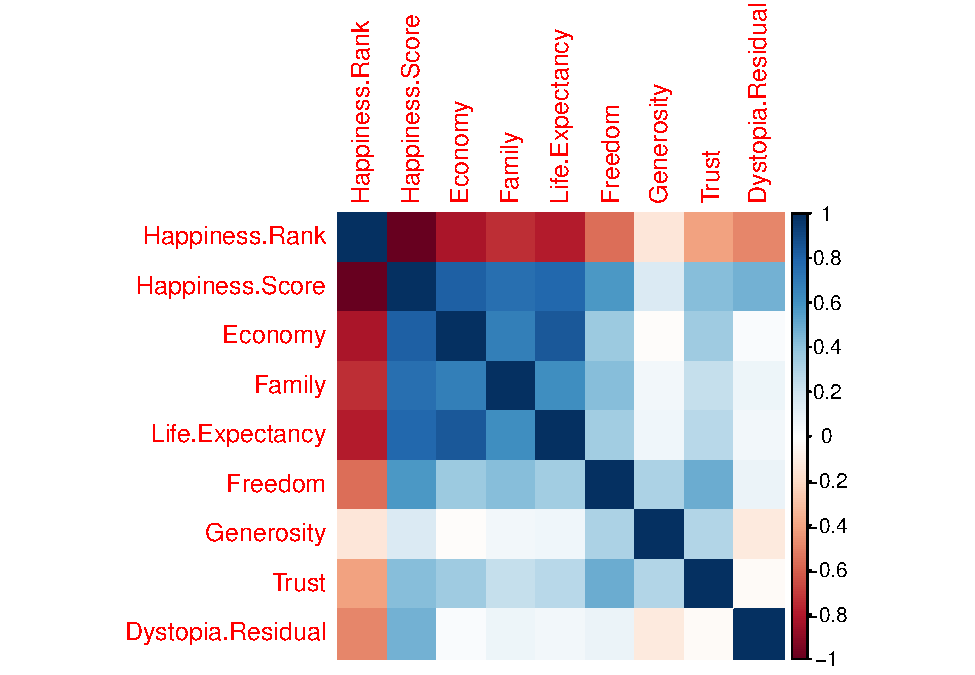
\includegraphics{Fer_files/figure-latex/unnamed-chunk-5-1.pdf}

Obviously, there is an inverse correlation between ``Happiness Rank''
and all the other numerical variables. In other words, the lower the
happiness rank, the higher the happiness score, and the higher the other
seven factors that contribute to happiness. So let's remove the
happiness rank, and see the correlation again.

\begin{Shaded}
\begin{Highlighting}[]
\CommentTok{\# Create a correlation plot}
\NormalTok{newdatacor }\OtherTok{=} \FunctionTok{cor}\NormalTok{(Happiness[}\FunctionTok{c}\NormalTok{(}\DecValTok{4}\SpecialCharTok{:}\DecValTok{11}\NormalTok{)])}
\FunctionTok{corrplot}\NormalTok{(newdatacor, }\AttributeTok{method =} \StringTok{"number"}\NormalTok{)}
\end{Highlighting}
\end{Shaded}

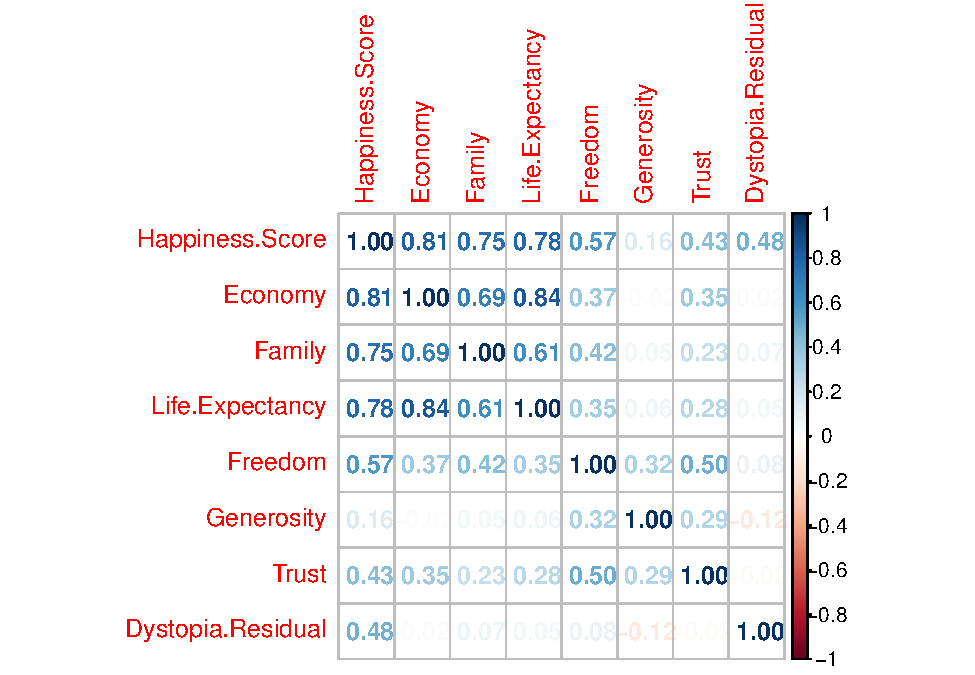
\includegraphics{Fer_files/figure-latex/unnamed-chunk-6-1.pdf}

According to the above cor plot, Economy, life expectancy, and family
play the most significant role in contributing to happiness. Trust and
generosity have the lowest impact on the happiness score.

\subsection{Comparing different continents regarding their happiness
variables}\label{comparing-different-continents-regarding-their-happiness-variables}

Let's calculate the average happiness score and the average of the other
seven variables for each continent. Then melt it to have variables and
values in separate columns. Finally, using ggplot to show the difference
between continents.

\begin{Shaded}
\begin{Highlighting}[]
\NormalTok{Happiness.Continent }\OtherTok{\textless{}{-}}\NormalTok{ Happiness }\SpecialCharTok{\%\textgreater{}\%}
                          \FunctionTok{select}\NormalTok{(}\SpecialCharTok{{-}}\DecValTok{3}\NormalTok{) }\SpecialCharTok{\%\textgreater{}\%}
                          \FunctionTok{group\_by}\NormalTok{(Continent) }\SpecialCharTok{\%\textgreater{}\%}
                          \FunctionTok{summarise\_at}\NormalTok{(}\FunctionTok{vars}\NormalTok{(}\SpecialCharTok{{-}}\NormalTok{Country), }\FunctionTok{funs}\NormalTok{(}\FunctionTok{mean}\NormalTok{(., }\AttributeTok{na.rm=}\ConstantTok{TRUE}\NormalTok{)))}

\CommentTok{\# Or we can use aggregate}
\CommentTok{\# aggregate(Happiness[, 4:11], list(Happiness$Continent), mean)}

\CommentTok{\# Melting the "Happiness.Continent" dataset}
\NormalTok{Happiness.Continent.melt }\OtherTok{\textless{}{-}} \FunctionTok{melt}\NormalTok{(Happiness.Continent)}


\CommentTok{\# Faceting}
\FunctionTok{ggplot}\NormalTok{(Happiness.Continent.melt, }\FunctionTok{aes}\NormalTok{(}\AttributeTok{y=}\NormalTok{value, }\AttributeTok{x=}\NormalTok{Continent, }\AttributeTok{color=}\NormalTok{Continent, }\AttributeTok{fill=}\NormalTok{Continent)) }\SpecialCharTok{+} 
  \FunctionTok{geom\_bar}\NormalTok{( }\AttributeTok{stat=}\StringTok{"identity"}\NormalTok{) }\SpecialCharTok{+}    
  \FunctionTok{facet\_wrap}\NormalTok{(}\SpecialCharTok{\textasciitilde{}}\NormalTok{variable) }\SpecialCharTok{+} \FunctionTok{theme\_bw}\NormalTok{() }\SpecialCharTok{+}
  \FunctionTok{theme}\NormalTok{(}\AttributeTok{axis.text.x =} \FunctionTok{element\_text}\NormalTok{(}\AttributeTok{angle =} \DecValTok{90}\NormalTok{, }\AttributeTok{hjust =} \DecValTok{1}\NormalTok{)) }\SpecialCharTok{+}
  \FunctionTok{labs}\NormalTok{(}\AttributeTok{title =} \StringTok{"Average value of happiness variables for different continents"}\NormalTok{, }
       \AttributeTok{y =} \StringTok{"Average value"}\NormalTok{) }
\end{Highlighting}
\end{Shaded}

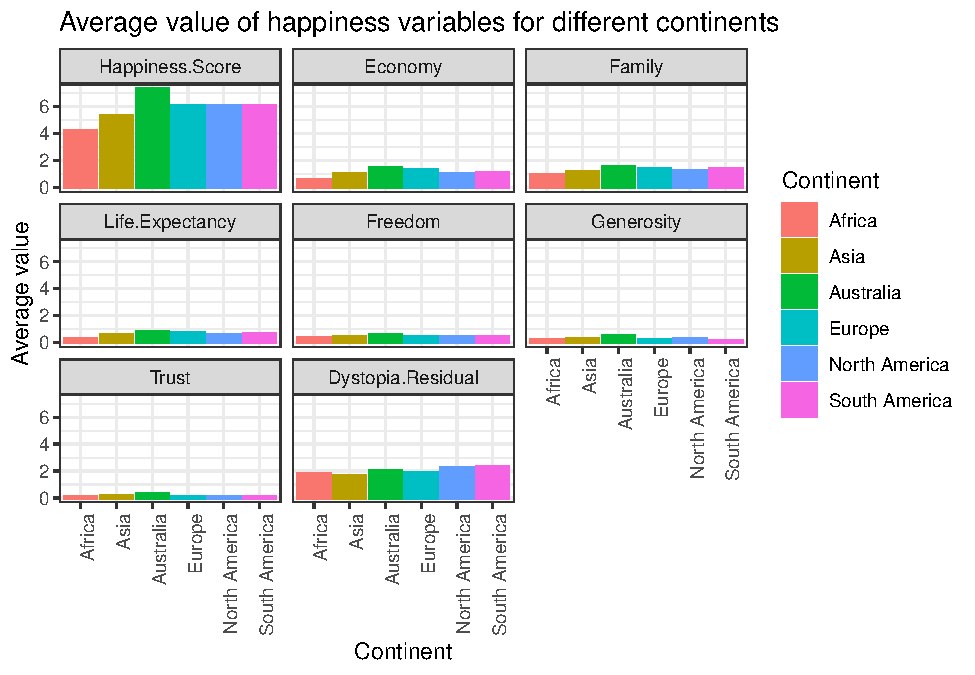
\includegraphics{Fer_files/figure-latex/unnamed-chunk-7-1.pdf}

We can see that Australia has approximately the highest average in all
fields except dystopia residual, after that Europe, North America, and
South America are roughly the same regarding happiness score and the
other seven factors. Finally, Asia and Africa have the lowest scores in
all fields.

\subsection{Correlation plot for each
continent}\label{correlation-plot-for-each-continent}

Let's see the correlation between variables for each continent.

\begin{Shaded}
\begin{Highlighting}[]
\FunctionTok{corrgram}\NormalTok{(Happiness }\SpecialCharTok{\%\textgreater{}\%} \FunctionTok{select}\NormalTok{(}\SpecialCharTok{{-}}\DecValTok{3}\NormalTok{) }\SpecialCharTok{\%\textgreater{}\%} \FunctionTok{filter}\NormalTok{(Continent }\SpecialCharTok{==} \StringTok{"Africa"}\NormalTok{), }\AttributeTok{order=}\ConstantTok{TRUE}\NormalTok{,}
         \AttributeTok{upper.panel=}\NormalTok{panel.cor, }\AttributeTok{main=}\StringTok{"Happiness Matrix for Africa"}\NormalTok{)}
\end{Highlighting}
\end{Shaded}

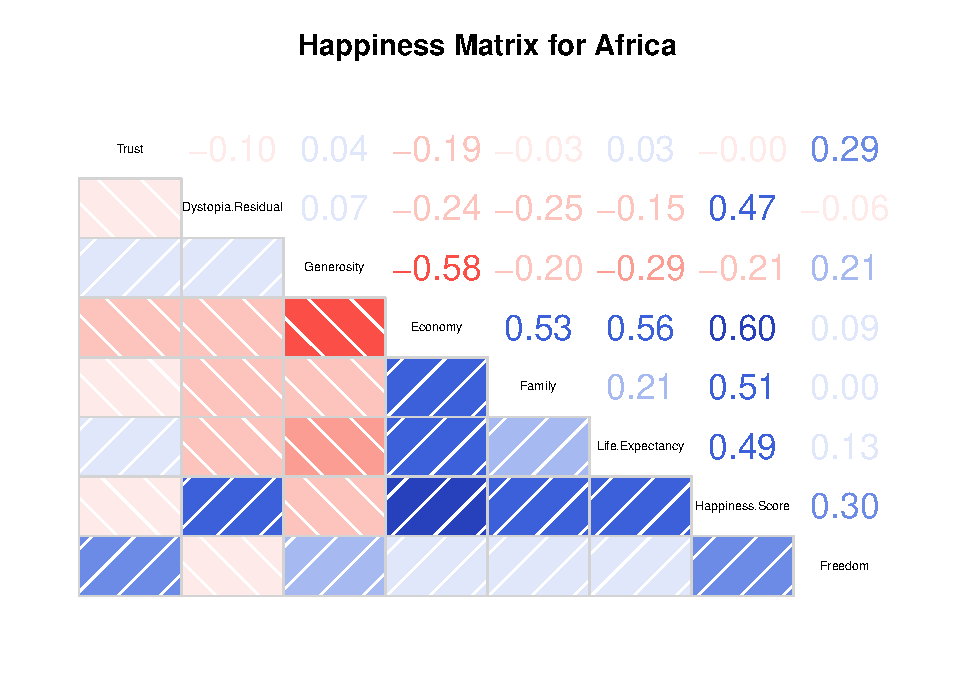
\includegraphics{Fer_files/figure-latex/unnamed-chunk-8-1.pdf}

\textbf{Correlation between ``Happiness Score'' and the other variables
in Africa:}\\
Economy \textgreater{} Family \textgreater{} Life.Expectancy
\textgreater{} Dystopia.Residual \textgreater{} Freedom\\
There is no correlation between happiness score and trust.\\
There is an inverse correlation between happiness score and generosity.

\begin{Shaded}
\begin{Highlighting}[]
\FunctionTok{corrgram}\NormalTok{(Happiness }\SpecialCharTok{\%\textgreater{}\%} \FunctionTok{select}\NormalTok{(}\SpecialCharTok{{-}}\DecValTok{3}\NormalTok{) }\SpecialCharTok{\%\textgreater{}\%} \FunctionTok{filter}\NormalTok{(Continent }\SpecialCharTok{==} \StringTok{"Asia"}\NormalTok{), }\AttributeTok{order=}\ConstantTok{TRUE}\NormalTok{,}
         \AttributeTok{upper.panel=}\NormalTok{panel.cor, }\AttributeTok{main=}\StringTok{"Happiness Matrix for Asia"}\NormalTok{)}
\end{Highlighting}
\end{Shaded}

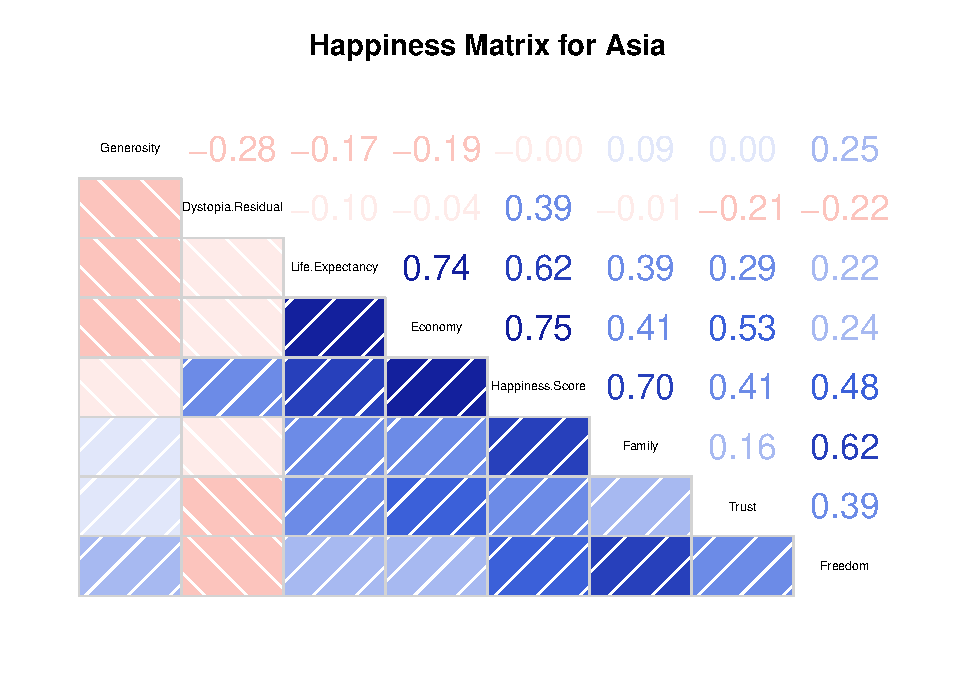
\includegraphics{Fer_files/figure-latex/unnamed-chunk-9-1.pdf}

\textbf{Correlation between ``Happiness Score'' and the other variables
in Asia:}\\
Economy \textgreater{} Family \textgreater{} Life.Expectancy
\textgreater{} Freedom \textgreater{} Trust \textgreater{}
Dystopia.Residual\\
There is no correlation between happiness score and generosity.

\begin{Shaded}
\begin{Highlighting}[]
\FunctionTok{corrgram}\NormalTok{(Happiness }\SpecialCharTok{\%\textgreater{}\%} \FunctionTok{select}\NormalTok{(}\SpecialCharTok{{-}}\DecValTok{3}\NormalTok{) }\SpecialCharTok{\%\textgreater{}\%} \FunctionTok{filter}\NormalTok{(Continent }\SpecialCharTok{==} \StringTok{"Europe"}\NormalTok{), }\AttributeTok{order=}\ConstantTok{TRUE}\NormalTok{,}
         \AttributeTok{upper.panel=}\NormalTok{panel.cor, }\AttributeTok{main=}\StringTok{"Happiness Matrix for Europe"}\NormalTok{)}
\end{Highlighting}
\end{Shaded}

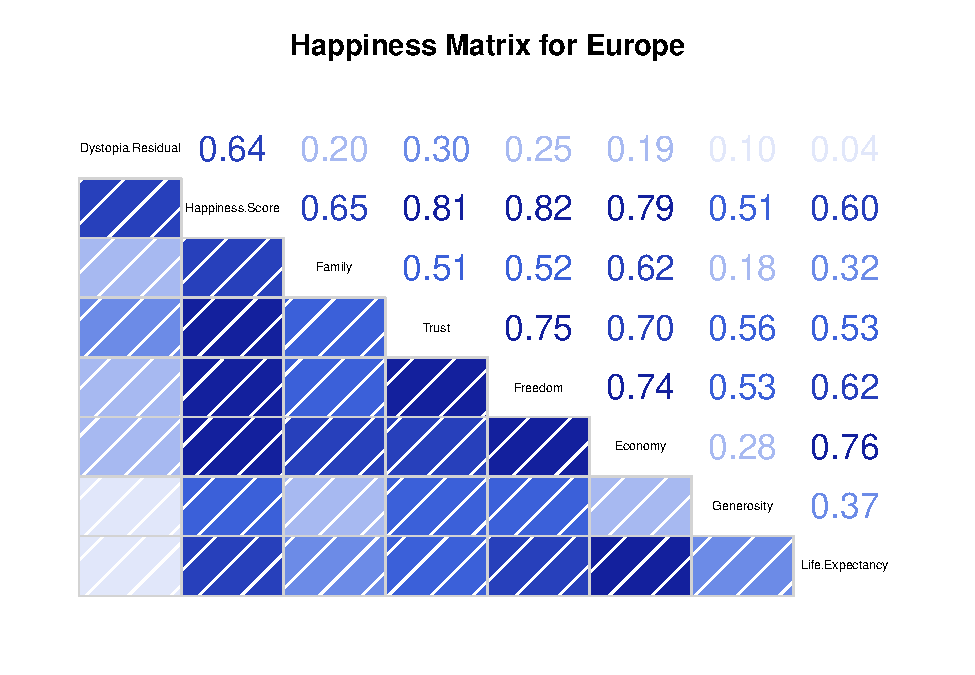
\includegraphics{Fer_files/figure-latex/unnamed-chunk-10-1.pdf}

\textbf{Correlation between ``Happiness Score'' and the other variables
in Europe:}\\
Freedom \textgreater{} Trust \textgreater{} Economy \textgreater{}
Family \textgreater{} Dystopia.Residual \textgreater{} Life.Expectancy
\textgreater{} Generosity\\
The highest correlation between generosity and happiness score took
place in Europe.

\begin{Shaded}
\begin{Highlighting}[]
\FunctionTok{corrgram}\NormalTok{(Happiness }\SpecialCharTok{\%\textgreater{}\%} \FunctionTok{select}\NormalTok{(}\SpecialCharTok{{-}}\DecValTok{3}\NormalTok{) }\SpecialCharTok{\%\textgreater{}\%} \FunctionTok{filter}\NormalTok{(Continent }\SpecialCharTok{==} \StringTok{"North America"}\NormalTok{), }\AttributeTok{order=}\ConstantTok{TRUE}\NormalTok{,}
         \AttributeTok{upper.panel=}\NormalTok{panel.cor, }\AttributeTok{main=}\StringTok{"Happiness Matrix for North America"}\NormalTok{)}
\end{Highlighting}
\end{Shaded}

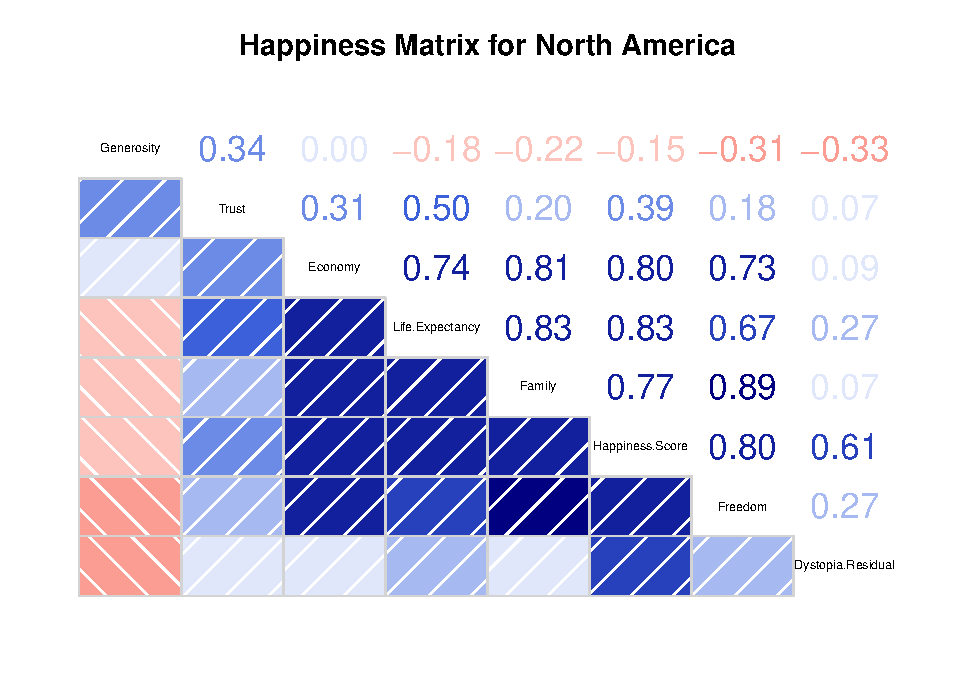
\includegraphics{Fer_files/figure-latex/unnamed-chunk-11-1.pdf}

\textbf{Correlation between ``Happiness Score'' and the other variables
in North America:}\\
Life.Expectancy \textgreater{} Economy \textgreater{} Freedom
\textgreater{} Family \textgreater{} Dystopia.Residual \textgreater{}
Trust\\
There is an inverse correlation between happiness score and generosity.

\begin{Shaded}
\begin{Highlighting}[]
\FunctionTok{corrgram}\NormalTok{(Happiness }\SpecialCharTok{\%\textgreater{}\%} \FunctionTok{select}\NormalTok{(}\SpecialCharTok{{-}}\DecValTok{3}\NormalTok{) }\SpecialCharTok{\%\textgreater{}\%} \FunctionTok{filter}\NormalTok{(Continent }\SpecialCharTok{==} \StringTok{"South America"}\NormalTok{), }\AttributeTok{order=}\ConstantTok{TRUE}\NormalTok{,}
         \AttributeTok{upper.panel=}\NormalTok{panel.cor, }\AttributeTok{main=}\StringTok{"Happiness Matrix for South America"}\NormalTok{)}
\end{Highlighting}
\end{Shaded}

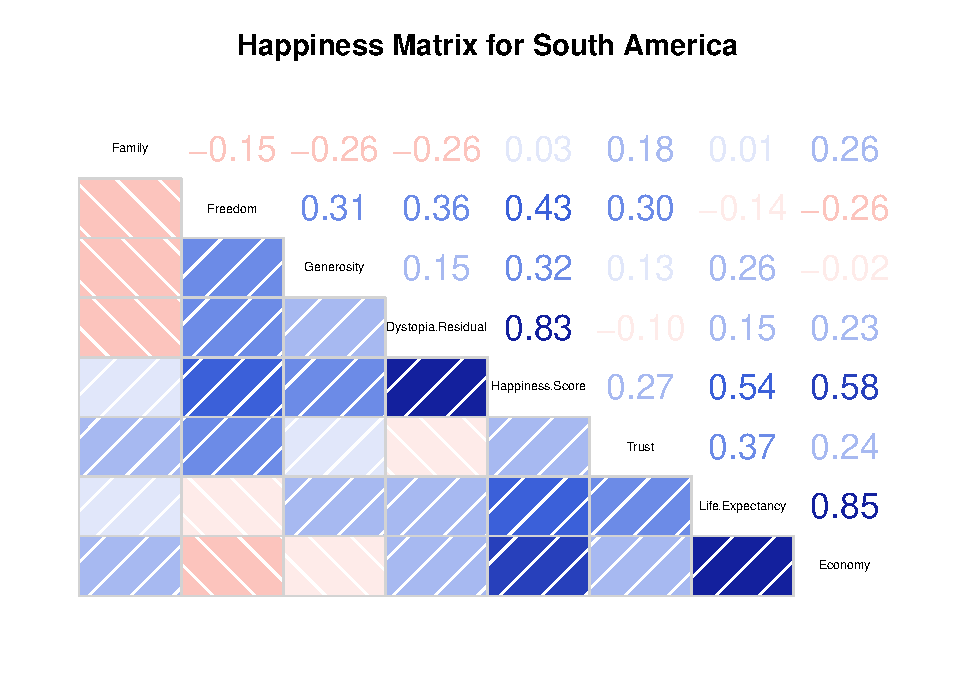
\includegraphics{Fer_files/figure-latex/unnamed-chunk-12-1.pdf}

\textbf{Correlation between ``Happiness Score'' and the other variables
in South America:}\\
Dystopia.Residual \textgreater{} Economy \textgreater{} Life.Expectancy
\textgreater{} Freedom \textgreater{} Generosity \textgreater{} Trust
\textgreater{} Family\\
The family is the least significant factor in South America.

\subsection{Happiness score comparison on different
continents}\label{happiness-score-comparison-on-different-continents}

We will use scatter plot, box plot, and violin plot to see the happiness
score distribution in different countries, how this score is populated
in these continents and also will calculate the mean and median of
happiness score for each of these continents.

\begin{Shaded}
\begin{Highlighting}[]
\DocumentationTok{\#\#\#\#\#\#\# Happiness score for each continent}

\NormalTok{gg1 }\OtherTok{\textless{}{-}} \FunctionTok{ggplot}\NormalTok{(Happiness,}
              \FunctionTok{aes}\NormalTok{(}\AttributeTok{x=}\NormalTok{Continent,}
                  \AttributeTok{y=}\NormalTok{Happiness.Score,}
                  \AttributeTok{color=}\NormalTok{Continent))}\SpecialCharTok{+}
  \FunctionTok{geom\_point}\NormalTok{() }\SpecialCharTok{+} \FunctionTok{theme\_bw}\NormalTok{() }\SpecialCharTok{+}
  \FunctionTok{theme}\NormalTok{(}\AttributeTok{axis.title =} \FunctionTok{element\_text}\NormalTok{(}\AttributeTok{family =} \StringTok{"Helvetica"}\NormalTok{, }\AttributeTok{size =}\NormalTok{ (}\DecValTok{8}\NormalTok{)))}

\NormalTok{gg2 }\OtherTok{\textless{}{-}} \FunctionTok{ggplot}\NormalTok{(Happiness , }\FunctionTok{aes}\NormalTok{(}\AttributeTok{x =}\NormalTok{ Continent, }\AttributeTok{y =}\NormalTok{ Happiness.Score)) }\SpecialCharTok{+}
  \FunctionTok{geom\_boxplot}\NormalTok{(}\FunctionTok{aes}\NormalTok{(}\AttributeTok{fill=}\NormalTok{Continent)) }\SpecialCharTok{+} \FunctionTok{theme\_bw}\NormalTok{() }\SpecialCharTok{+}
  \FunctionTok{theme}\NormalTok{(}\AttributeTok{axis.title =} \FunctionTok{element\_text}\NormalTok{(}\AttributeTok{family =} \StringTok{"Helvetica"}\NormalTok{, }\AttributeTok{size =}\NormalTok{ (}\DecValTok{8}\NormalTok{)))}

\NormalTok{gg3 }\OtherTok{\textless{}{-}} \FunctionTok{ggplot}\NormalTok{(Happiness,}\FunctionTok{aes}\NormalTok{(}\AttributeTok{x=}\NormalTok{Continent,}\AttributeTok{y=}\NormalTok{Happiness.Score))}\SpecialCharTok{+}
  \FunctionTok{geom\_violin}\NormalTok{(}\FunctionTok{aes}\NormalTok{(}\AttributeTok{fill=}\NormalTok{Continent),}\AttributeTok{alpha=}\FloatTok{0.7}\NormalTok{)}\SpecialCharTok{+} \FunctionTok{theme\_bw}\NormalTok{() }\SpecialCharTok{+}
  \FunctionTok{theme}\NormalTok{(}\AttributeTok{axis.title =} \FunctionTok{element\_text}\NormalTok{(}\AttributeTok{family =} \StringTok{"Helvetica"}\NormalTok{, }\AttributeTok{size =}\NormalTok{ (}\DecValTok{8}\NormalTok{)))}

\CommentTok{\# Compute descriptive statistics by groups}
\NormalTok{stable }\OtherTok{\textless{}{-}} \FunctionTok{desc\_statby}\NormalTok{(Happiness, }\AttributeTok{measure.var =} \StringTok{"Happiness.Score"}\NormalTok{,}
                      \AttributeTok{grps =} \StringTok{"Continent"}\NormalTok{)}
\NormalTok{stable }\OtherTok{\textless{}{-}}\NormalTok{ stable[, }\FunctionTok{c}\NormalTok{(}\StringTok{"Continent"}\NormalTok{,}\StringTok{"mean"}\NormalTok{,}\StringTok{"median"}\NormalTok{)]}
\FunctionTok{names}\NormalTok{(stable) }\OtherTok{\textless{}{-}} \FunctionTok{c}\NormalTok{(}\StringTok{"Continent"}\NormalTok{, }\StringTok{"Mean of happiness score"}\NormalTok{,}\StringTok{"Median of happiness score"}\NormalTok{)}
\CommentTok{\# Summary table plot}
\NormalTok{stable.p }\OtherTok{\textless{}{-}} \FunctionTok{ggtexttable}\NormalTok{(stable,}\AttributeTok{rows =} \ConstantTok{NULL}\NormalTok{, }
                         \AttributeTok{theme =} \FunctionTok{ttheme}\NormalTok{(}\StringTok{"classic"}\NormalTok{))}


\FunctionTok{ggarrange}\NormalTok{(gg1, gg2, }\AttributeTok{ncol =} \DecValTok{1}\NormalTok{, }\AttributeTok{nrow =} \DecValTok{2}\NormalTok{)}
\end{Highlighting}
\end{Shaded}

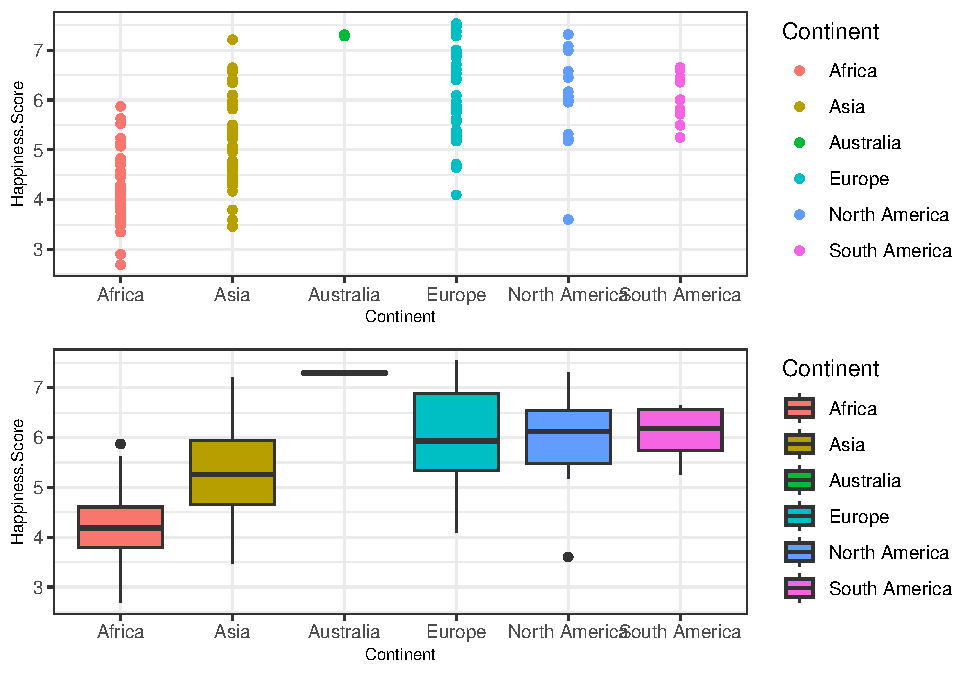
\includegraphics{Fer_files/figure-latex/unnamed-chunk-13-1.pdf}

\begin{Shaded}
\begin{Highlighting}[]
\FunctionTok{ggarrange}\NormalTok{(gg3, stable.p, }\AttributeTok{ncol =} \DecValTok{1}\NormalTok{, }\AttributeTok{nrow =} \DecValTok{2}\NormalTok{)}
\end{Highlighting}
\end{Shaded}

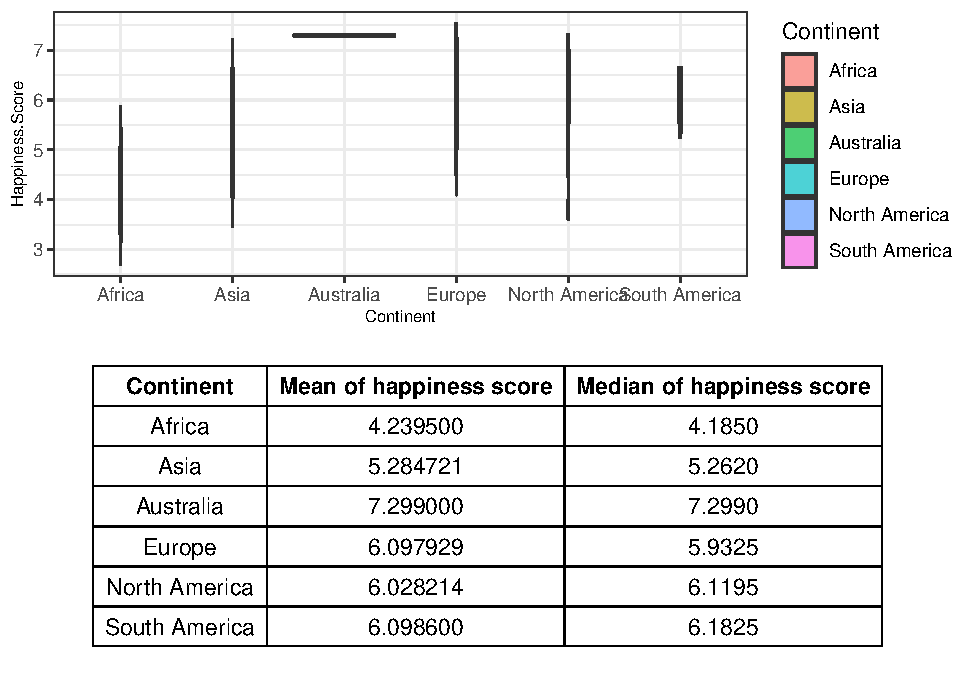
\includegraphics{Fer_files/figure-latex/unnamed-chunk-13-2.pdf}

As we have seen before, Australia has the highest median happiness
score. Europe, South America, and North America are in the second place
regarding median happiness score. Asia has the lowest median after
Africa. We can see the range of happiness score for different
continents, and also the concentration of happiness score.

\subsection{Scatter plot with regression
line}\label{scatter-plot-with-regression-line}

Let's see the correlation between happiness score and the other seven
factors in the happiness dataset for different continents by creating a
scatter plot.

\begin{Shaded}
\begin{Highlighting}[]
\FunctionTok{ggplot}\NormalTok{(}\FunctionTok{subset}\NormalTok{(Happiness, Happiness}\SpecialCharTok{$}\NormalTok{Continent }\SpecialCharTok{!=} \StringTok{"Australia"}\NormalTok{), }\FunctionTok{aes}\NormalTok{(}\AttributeTok{x =}\NormalTok{ Life.Expectancy, }\AttributeTok{y =}\NormalTok{ Happiness.Score)) }\SpecialCharTok{+} 
  \FunctionTok{geom\_point}\NormalTok{(}\FunctionTok{aes}\NormalTok{(}\AttributeTok{color=}\NormalTok{Continent), }\AttributeTok{size =} \DecValTok{3}\NormalTok{, }\AttributeTok{alpha =} \FloatTok{0.8}\NormalTok{) }\SpecialCharTok{+}  
  \FunctionTok{geom\_smooth}\NormalTok{(}\FunctionTok{aes}\NormalTok{(}\AttributeTok{color =}\NormalTok{ Continent, }\AttributeTok{fill =}\NormalTok{ Continent), }
              \AttributeTok{method =} \StringTok{"lm"}\NormalTok{, }\AttributeTok{fullrange =} \ConstantTok{TRUE}\NormalTok{) }\SpecialCharTok{+}
  \FunctionTok{facet\_wrap}\NormalTok{(}\SpecialCharTok{\textasciitilde{}}\NormalTok{Continent) }\SpecialCharTok{+}
  \FunctionTok{theme\_bw}\NormalTok{() }\SpecialCharTok{+} \FunctionTok{labs}\NormalTok{(}\AttributeTok{title =} \StringTok{"Scatter plot with regression line"}\NormalTok{)}
\end{Highlighting}
\end{Shaded}

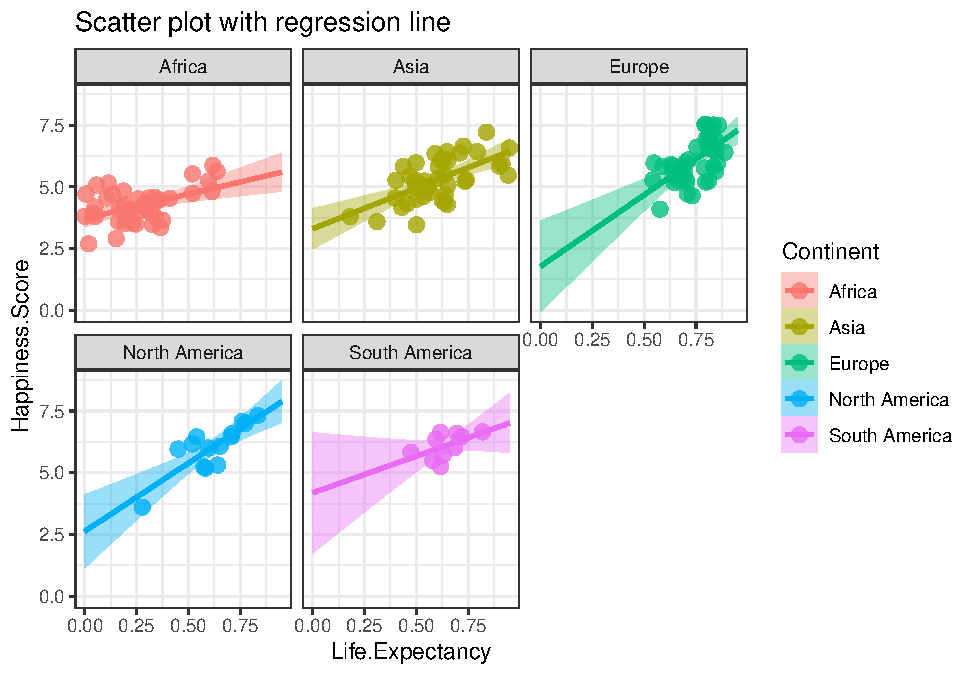
\includegraphics{Fer_files/figure-latex/unnamed-chunk-14-1.pdf}

The correlation between life expectancy and happiness score in Europe,
North America, and Asia is more significant than the other continents.
Worth mentioning that we will not take Australia into account because
there are just two countries in Australia and creating scatter plot with
the regression line for this continent will not give us any insight.

\begin{Shaded}
\begin{Highlighting}[]
\FunctionTok{ggplot}\NormalTok{(}\FunctionTok{subset}\NormalTok{(Happiness, Happiness}\SpecialCharTok{$}\NormalTok{Continent }\SpecialCharTok{!=} \StringTok{"Australia"}\NormalTok{), }\FunctionTok{aes}\NormalTok{(}\AttributeTok{x =}\NormalTok{ Economy, }\AttributeTok{y =}\NormalTok{ Happiness.Score)) }\SpecialCharTok{+} 
  \FunctionTok{geom\_point}\NormalTok{(}\FunctionTok{aes}\NormalTok{(}\AttributeTok{color=}\NormalTok{Continent), }\AttributeTok{size =} \DecValTok{3}\NormalTok{, }\AttributeTok{alpha =} \FloatTok{0.8}\NormalTok{) }\SpecialCharTok{+}  
  \FunctionTok{geom\_smooth}\NormalTok{(}\FunctionTok{aes}\NormalTok{(}\AttributeTok{color =}\NormalTok{ Continent, }\AttributeTok{fill =}\NormalTok{ Continent), }
              \AttributeTok{method =} \StringTok{"lm"}\NormalTok{, }\AttributeTok{fullrange =} \ConstantTok{TRUE}\NormalTok{) }\SpecialCharTok{+}
  \FunctionTok{facet\_wrap}\NormalTok{(}\SpecialCharTok{\textasciitilde{}}\NormalTok{Continent) }\SpecialCharTok{+}
  \FunctionTok{theme\_bw}\NormalTok{() }\SpecialCharTok{+} \FunctionTok{labs}\NormalTok{(}\AttributeTok{title =} \StringTok{"Scatter plot with regression line"}\NormalTok{)}
\end{Highlighting}
\end{Shaded}

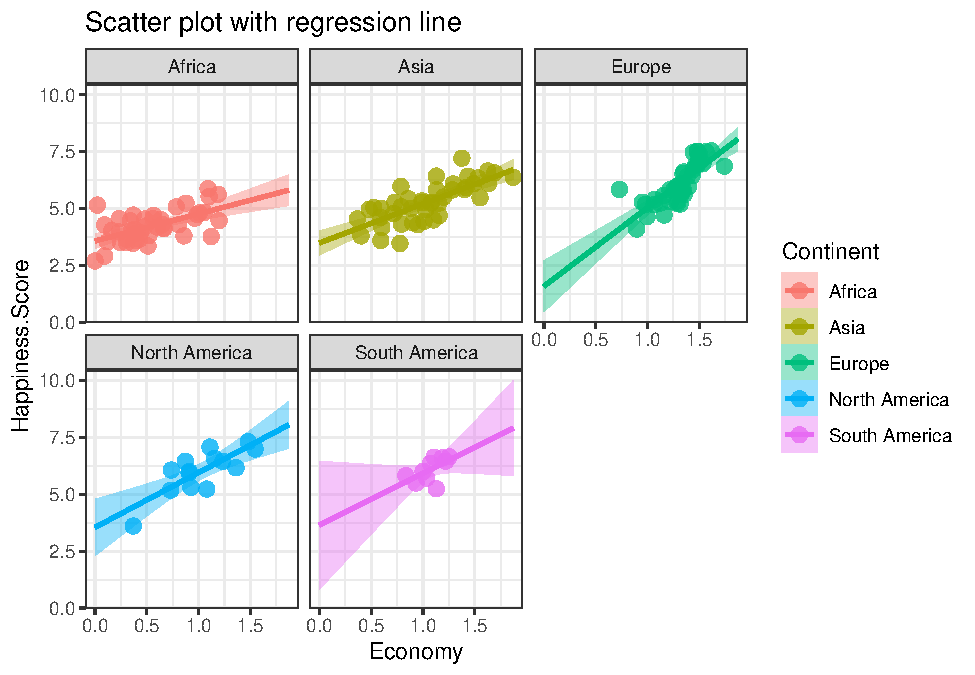
\includegraphics{Fer_files/figure-latex/unnamed-chunk-15-1.pdf}

We can see pretty the same result here for the correlation between
happiness score and economy. Africa has the lowest relationship in this
regard.

\begin{Shaded}
\begin{Highlighting}[]
\FunctionTok{ggplot}\NormalTok{(}\FunctionTok{subset}\NormalTok{(Happiness, Happiness}\SpecialCharTok{$}\NormalTok{Continent }\SpecialCharTok{!=} \StringTok{"Australia"}\NormalTok{), }\FunctionTok{aes}\NormalTok{(}\AttributeTok{x =}\NormalTok{ Freedom, }\AttributeTok{y =}\NormalTok{ Happiness.Score)) }\SpecialCharTok{+} 
  \FunctionTok{geom\_point}\NormalTok{(}\FunctionTok{aes}\NormalTok{(}\AttributeTok{color=}\NormalTok{Continent), }\AttributeTok{size =} \DecValTok{3}\NormalTok{, }\AttributeTok{alpha =} \FloatTok{0.8}\NormalTok{) }\SpecialCharTok{+}  
  \FunctionTok{geom\_smooth}\NormalTok{(}\FunctionTok{aes}\NormalTok{(}\AttributeTok{color =}\NormalTok{ Continent, }\AttributeTok{fill =}\NormalTok{ Continent), }
              \AttributeTok{method =} \StringTok{"lm"}\NormalTok{, }\AttributeTok{fullrange =} \ConstantTok{TRUE}\NormalTok{) }\SpecialCharTok{+}
  \FunctionTok{facet\_wrap}\NormalTok{(}\SpecialCharTok{\textasciitilde{}}\NormalTok{Continent) }\SpecialCharTok{+}
  \FunctionTok{theme\_bw}\NormalTok{() }\SpecialCharTok{+} \FunctionTok{labs}\NormalTok{(}\AttributeTok{title =} \StringTok{"Scatter plot with regression line"}\NormalTok{)}
\end{Highlighting}
\end{Shaded}

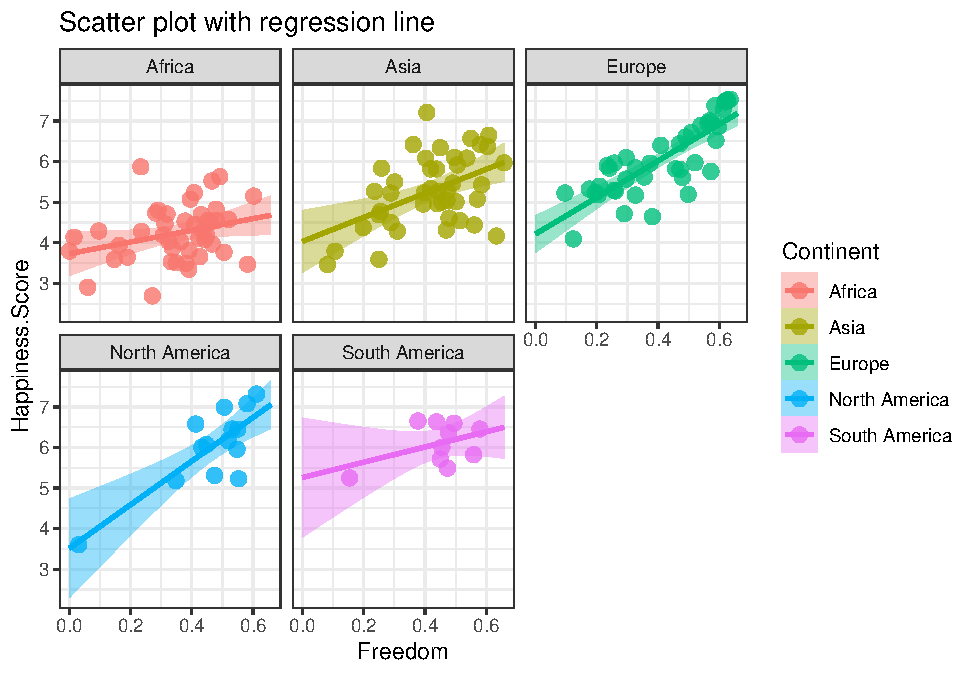
\includegraphics{Fer_files/figure-latex/unnamed-chunk-16-1.pdf}

Freedom in Europe and North America is more correlated to happiness
score than any other continents.

\begin{Shaded}
\begin{Highlighting}[]
\FunctionTok{ggplot}\NormalTok{(}\FunctionTok{subset}\NormalTok{(Happiness, Happiness}\SpecialCharTok{$}\NormalTok{Continent }\SpecialCharTok{!=} \StringTok{"Australia"}\NormalTok{), }\FunctionTok{aes}\NormalTok{(}\AttributeTok{x =}\NormalTok{ Trust, }\AttributeTok{y =}\NormalTok{ Happiness.Score)) }\SpecialCharTok{+} 
  \FunctionTok{geom\_point}\NormalTok{(}\FunctionTok{aes}\NormalTok{(}\AttributeTok{color=}\NormalTok{Continent), }\AttributeTok{size =} \DecValTok{3}\NormalTok{, }\AttributeTok{alpha =} \FloatTok{0.8}\NormalTok{) }\SpecialCharTok{+}  
  \FunctionTok{geom\_smooth}\NormalTok{(}\FunctionTok{aes}\NormalTok{(}\AttributeTok{color =}\NormalTok{ Continent, }\AttributeTok{fill =}\NormalTok{ Continent), }
              \AttributeTok{method =} \StringTok{"lm"}\NormalTok{, }\AttributeTok{fullrange =} \ConstantTok{TRUE}\NormalTok{) }\SpecialCharTok{+}
  \FunctionTok{facet\_wrap}\NormalTok{(}\SpecialCharTok{\textasciitilde{}}\NormalTok{Continent) }\SpecialCharTok{+}
  \FunctionTok{theme\_bw}\NormalTok{() }\SpecialCharTok{+} \FunctionTok{labs}\NormalTok{(}\AttributeTok{title =} \StringTok{"Scatter plot with regression line"}\NormalTok{)}
\end{Highlighting}
\end{Shaded}

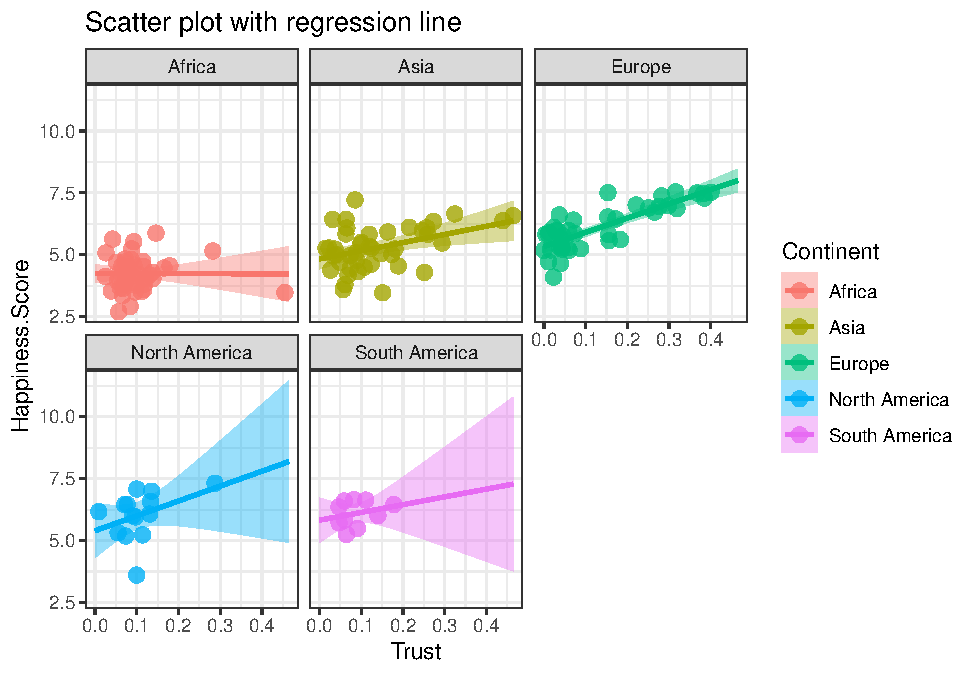
\includegraphics{Fer_files/figure-latex/unnamed-chunk-17-1.pdf}

Approximately there is no correlation between trust and happiness score
in Africa.

\begin{Shaded}
\begin{Highlighting}[]
\FunctionTok{ggplot}\NormalTok{(}\FunctionTok{subset}\NormalTok{(Happiness, Happiness}\SpecialCharTok{$}\NormalTok{Continent }\SpecialCharTok{!=} \StringTok{"Australia"}\NormalTok{), }\FunctionTok{aes}\NormalTok{(}\AttributeTok{x =}\NormalTok{ Generosity, }\AttributeTok{y =}\NormalTok{ Happiness.Score)) }\SpecialCharTok{+} 
  \FunctionTok{geom\_point}\NormalTok{(}\FunctionTok{aes}\NormalTok{(}\AttributeTok{color=}\NormalTok{Continent), }\AttributeTok{size =} \DecValTok{3}\NormalTok{, }\AttributeTok{alpha =} \FloatTok{0.8}\NormalTok{) }\SpecialCharTok{+}  
  \FunctionTok{geom\_smooth}\NormalTok{(}\FunctionTok{aes}\NormalTok{(}\AttributeTok{color =}\NormalTok{ Continent, }\AttributeTok{fill =}\NormalTok{ Continent), }
              \AttributeTok{method =} \StringTok{"lm"}\NormalTok{, }\AttributeTok{fullrange =} \ConstantTok{TRUE}\NormalTok{) }\SpecialCharTok{+}
  \FunctionTok{facet\_wrap}\NormalTok{(}\SpecialCharTok{\textasciitilde{}}\NormalTok{Continent) }\SpecialCharTok{+}
  \FunctionTok{theme\_bw}\NormalTok{() }\SpecialCharTok{+} \FunctionTok{labs}\NormalTok{(}\AttributeTok{title =} \StringTok{"Scatter plot with regression line"}\NormalTok{)}
\end{Highlighting}
\end{Shaded}

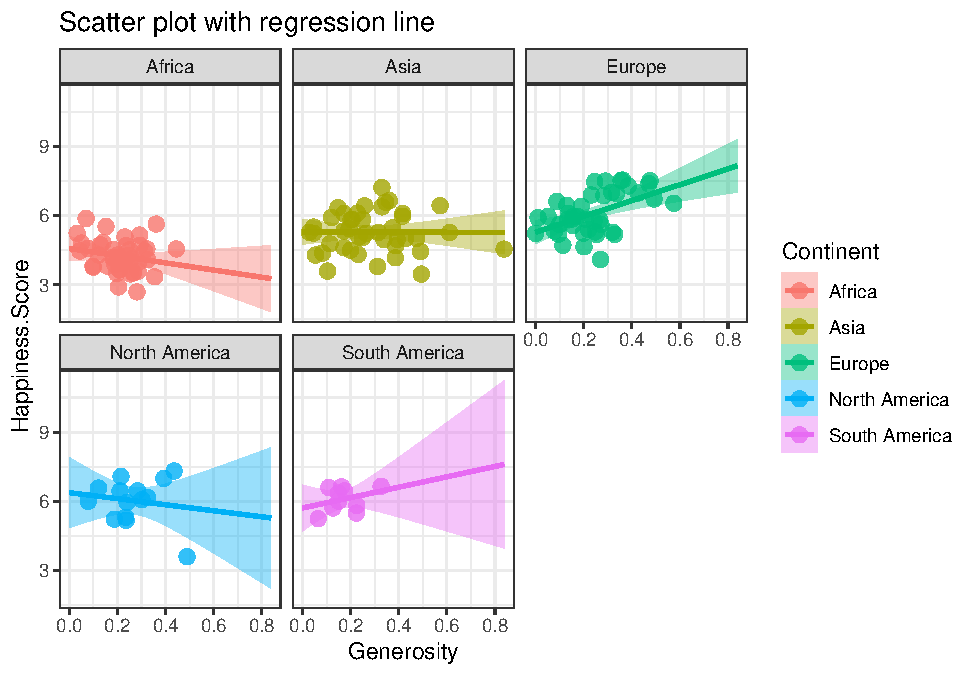
\includegraphics{Fer_files/figure-latex/unnamed-chunk-18-1.pdf}

The regression line has a positive slope only for Europe and South
America. For Asia the line is horizontal, and for Africa and North
America the slope is negative.

\begin{Shaded}
\begin{Highlighting}[]
\FunctionTok{ggplot}\NormalTok{(}\FunctionTok{subset}\NormalTok{(Happiness, Happiness}\SpecialCharTok{$}\NormalTok{Continent }\SpecialCharTok{!=} \StringTok{"Australia"}\NormalTok{), }\FunctionTok{aes}\NormalTok{(}\AttributeTok{x =}\NormalTok{ Family, }\AttributeTok{y =}\NormalTok{ Happiness.Score)) }\SpecialCharTok{+} 
  \FunctionTok{geom\_point}\NormalTok{(}\FunctionTok{aes}\NormalTok{(}\AttributeTok{color=}\NormalTok{Continent), }\AttributeTok{size =} \DecValTok{3}\NormalTok{, }\AttributeTok{alpha =} \FloatTok{0.8}\NormalTok{) }\SpecialCharTok{+}  
  \FunctionTok{geom\_smooth}\NormalTok{(}\FunctionTok{aes}\NormalTok{(}\AttributeTok{color =}\NormalTok{ Continent, }\AttributeTok{fill =}\NormalTok{ Continent), }
              \AttributeTok{method =} \StringTok{"lm"}\NormalTok{, }\AttributeTok{fullrange =} \ConstantTok{TRUE}\NormalTok{) }\SpecialCharTok{+}
  \FunctionTok{facet\_wrap}\NormalTok{(}\SpecialCharTok{\textasciitilde{}}\NormalTok{Continent) }\SpecialCharTok{+}
  \FunctionTok{theme\_bw}\NormalTok{() }\SpecialCharTok{+} \FunctionTok{labs}\NormalTok{(}\AttributeTok{title =} \StringTok{"Scatter plot with regression line"}\NormalTok{)}
\end{Highlighting}
\end{Shaded}

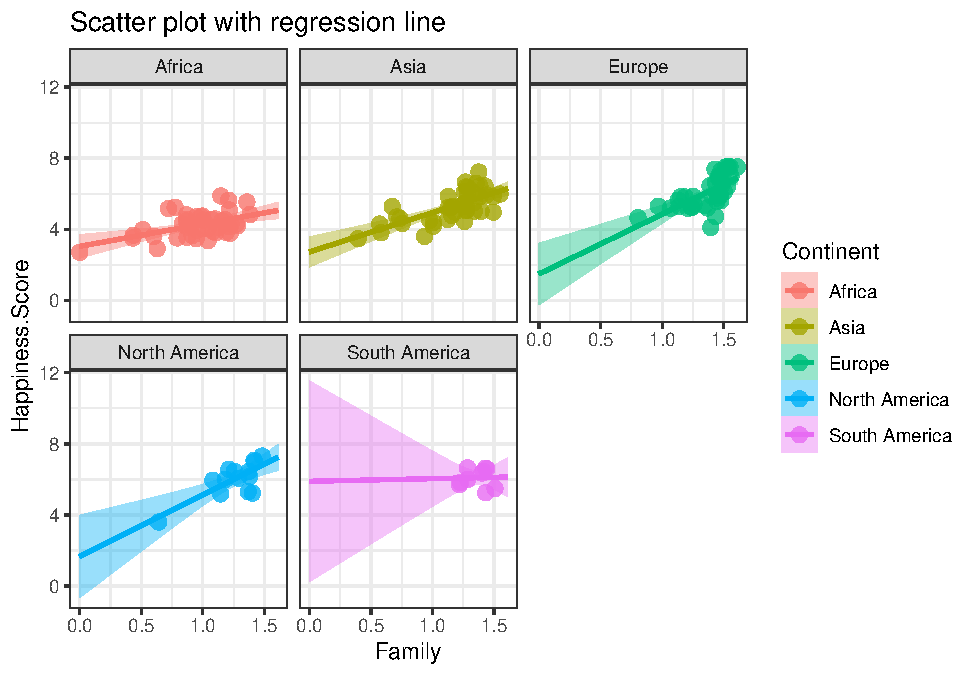
\includegraphics{Fer_files/figure-latex/unnamed-chunk-19-1.pdf}

In South America with increase in the family score, the happiness score
remains constant.

\begin{Shaded}
\begin{Highlighting}[]
\FunctionTok{ggplot}\NormalTok{(}\FunctionTok{subset}\NormalTok{(Happiness, Happiness}\SpecialCharTok{$}\NormalTok{Continent }\SpecialCharTok{!=} \StringTok{"Australia"}\NormalTok{), }\FunctionTok{aes}\NormalTok{(}\AttributeTok{x =}\NormalTok{ Dystopia.Residual, }\AttributeTok{y =}\NormalTok{ Happiness.Score)) }\SpecialCharTok{+} 
  \FunctionTok{geom\_point}\NormalTok{(}\FunctionTok{aes}\NormalTok{(}\AttributeTok{color=}\NormalTok{Continent), }\AttributeTok{size =} \DecValTok{3}\NormalTok{, }\AttributeTok{alpha =} \FloatTok{0.8}\NormalTok{) }\SpecialCharTok{+}  
  \FunctionTok{geom\_smooth}\NormalTok{(}\FunctionTok{aes}\NormalTok{(}\AttributeTok{color =}\NormalTok{ Continent, }\AttributeTok{fill =}\NormalTok{ Continent), }
              \AttributeTok{method =} \StringTok{"lm"}\NormalTok{, }\AttributeTok{fullrange =} \ConstantTok{TRUE}\NormalTok{) }\SpecialCharTok{+}
  \FunctionTok{facet\_wrap}\NormalTok{(}\SpecialCharTok{\textasciitilde{}}\NormalTok{Continent) }\SpecialCharTok{+}
  \FunctionTok{theme\_bw}\NormalTok{() }\SpecialCharTok{+} \FunctionTok{labs}\NormalTok{(}\AttributeTok{title =} \StringTok{"Scatter plot with regression line"}\NormalTok{)}
\end{Highlighting}
\end{Shaded}

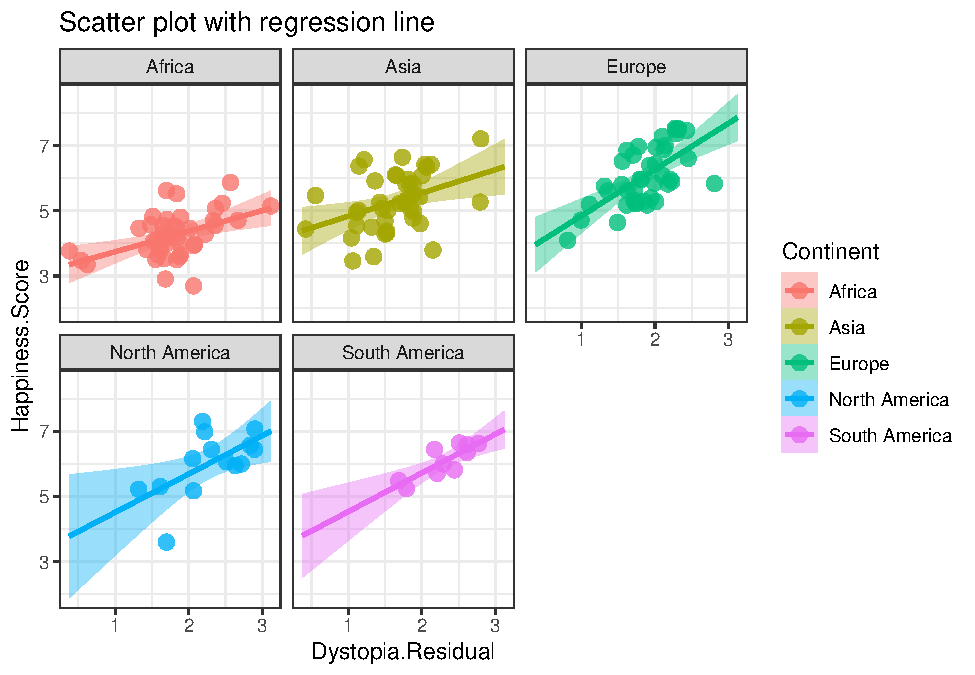
\includegraphics{Fer_files/figure-latex/unnamed-chunk-20-1.pdf}

All continents act pretty the same regarding dystopia residual.

\subsection{Scatter plot colored by
Continents}\label{scatter-plot-colored-by-continents}

The following is just another way of seeing happiness score distribution
on different continents when taking the correlation of happiness score
with different variables into account.

\begin{Shaded}
\begin{Highlighting}[]
\CommentTok{\#::::::::::::::::::::::::::::Generosity::::::::::::::::::::::::::::::}
\NormalTok{sp }\OtherTok{\textless{}{-}} \FunctionTok{ggscatter}\NormalTok{(Happiness, }\AttributeTok{x =} \StringTok{"Generosity"}\NormalTok{, }\AttributeTok{y =} \StringTok{"Happiness.Score"}\NormalTok{,}
                \AttributeTok{color =} \StringTok{"Continent"}\NormalTok{, }\AttributeTok{palette =} \StringTok{"jco"}\NormalTok{,}
                \AttributeTok{size =} \DecValTok{3}\NormalTok{, }\AttributeTok{alpha =} \FloatTok{0.6}\NormalTok{)}
\CommentTok{\# Create box plots of x/y variables}
\CommentTok{\# Box plot of the x variable}
\NormalTok{xbp }\OtherTok{\textless{}{-}} \FunctionTok{ggboxplot}\NormalTok{(Happiness}\SpecialCharTok{$}\NormalTok{Generosity, }\AttributeTok{width =} \FloatTok{0.3}\NormalTok{, }\AttributeTok{fill =} \StringTok{"lightgray"}\NormalTok{) }\SpecialCharTok{+}
  \FunctionTok{rotate}\NormalTok{() }\SpecialCharTok{+}
  \FunctionTok{theme\_transparent}\NormalTok{()}
\CommentTok{\# Box plot of the y variable}
\NormalTok{ybp }\OtherTok{\textless{}{-}} \FunctionTok{ggboxplot}\NormalTok{(Happiness}\SpecialCharTok{$}\NormalTok{Happiness.Score, }\AttributeTok{width =} \FloatTok{0.3}\NormalTok{, }\AttributeTok{fill =} \StringTok{"lightgray"}\NormalTok{) }\SpecialCharTok{+}
  \FunctionTok{theme\_transparent}\NormalTok{()}
\CommentTok{\# Create the external graphical objects}
\CommentTok{\# called a "grop" in Grid terminology}
\NormalTok{xbp\_grob }\OtherTok{\textless{}{-}} \FunctionTok{ggplotGrob}\NormalTok{(xbp)}
\NormalTok{ybp\_grob }\OtherTok{\textless{}{-}} \FunctionTok{ggplotGrob}\NormalTok{(ybp)}
\CommentTok{\# Place box plots inside the scatter plot}
\NormalTok{xmin }\OtherTok{\textless{}{-}} \FunctionTok{min}\NormalTok{(Happiness}\SpecialCharTok{$}\NormalTok{Generosity); xmax }\OtherTok{\textless{}{-}} \FunctionTok{max}\NormalTok{(Happiness}\SpecialCharTok{$}\NormalTok{Generosity)}
\NormalTok{ymin }\OtherTok{\textless{}{-}} \FunctionTok{min}\NormalTok{(Happiness}\SpecialCharTok{$}\NormalTok{Happiness.Score); ymax }\OtherTok{\textless{}{-}} \FunctionTok{max}\NormalTok{(Happiness}\SpecialCharTok{$}\NormalTok{Happiness.Score)}
\NormalTok{yoffset }\OtherTok{\textless{}{-}}\NormalTok{ (}\DecValTok{1}\SpecialCharTok{/}\DecValTok{15}\NormalTok{)}\SpecialCharTok{*}\NormalTok{ymax; xoffset }\OtherTok{\textless{}{-}}\NormalTok{ (}\DecValTok{1}\SpecialCharTok{/}\DecValTok{15}\NormalTok{)}\SpecialCharTok{*}\NormalTok{xmax}
\CommentTok{\# Insert xbp\_grob inside the scatter plot}
\NormalTok{sp }\SpecialCharTok{+} \FunctionTok{annotation\_custom}\NormalTok{(}\AttributeTok{grob =}\NormalTok{ xbp\_grob, }\AttributeTok{xmin =}\NormalTok{ xmin, }\AttributeTok{xmax =}\NormalTok{ xmax, }
                       \AttributeTok{ymin =}\NormalTok{ ymin}\SpecialCharTok{{-}}\NormalTok{yoffset, }\AttributeTok{ymax =}\NormalTok{ ymin}\SpecialCharTok{+}\NormalTok{yoffset) }\SpecialCharTok{+}
  \CommentTok{\# Insert ybp\_grob inside the scatter plot}
  \FunctionTok{annotation\_custom}\NormalTok{(}\AttributeTok{grob =}\NormalTok{ ybp\_grob,}
                    \AttributeTok{xmin =}\NormalTok{ xmin}\SpecialCharTok{{-}}\NormalTok{xoffset, }\AttributeTok{xmax =}\NormalTok{ xmin}\SpecialCharTok{+}\NormalTok{xoffset, }
                    \AttributeTok{ymin =}\NormalTok{ ymin, }\AttributeTok{ymax =}\NormalTok{ ymax)}
\end{Highlighting}
\end{Shaded}

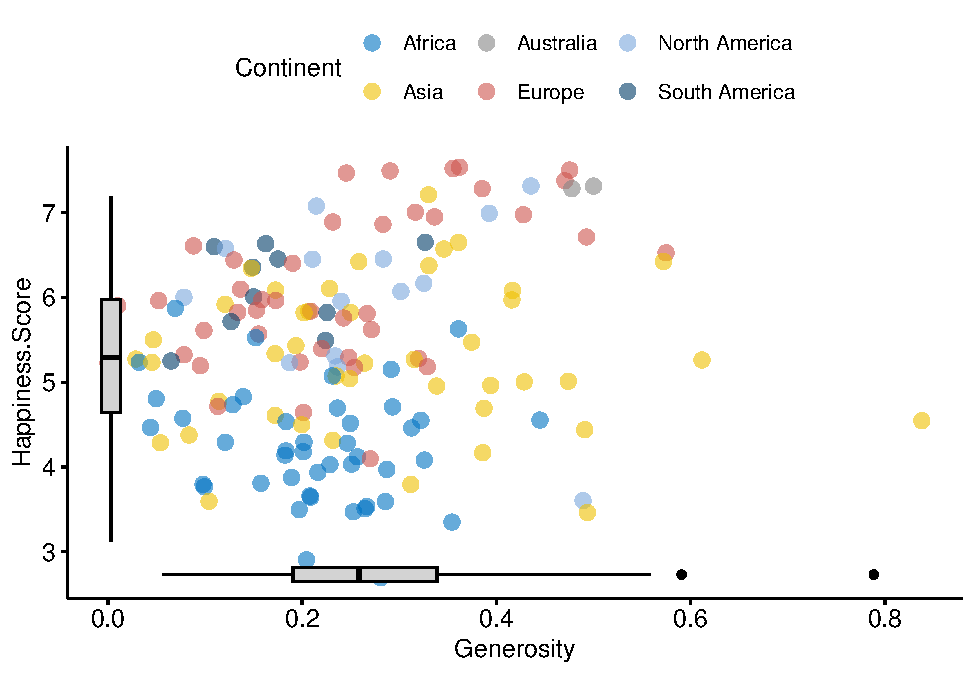
\includegraphics{Fer_files/figure-latex/unnamed-chunk-21-1.pdf}

\begin{Shaded}
\begin{Highlighting}[]
\CommentTok{\#::::::::::::::::::::::::::::Family::::::::::::::::::::::::::::::}
\NormalTok{sp }\OtherTok{\textless{}{-}} \FunctionTok{ggscatter}\NormalTok{(Happiness, }\AttributeTok{x =} \StringTok{"Family"}\NormalTok{, }\AttributeTok{y =} \StringTok{"Happiness.Score"}\NormalTok{,}
                \AttributeTok{color =} \StringTok{"Continent"}\NormalTok{, }\AttributeTok{palette =} \StringTok{"jco"}\NormalTok{,}
                \AttributeTok{size =} \DecValTok{3}\NormalTok{, }\AttributeTok{alpha =} \FloatTok{0.6}\NormalTok{)}
\CommentTok{\# Create box plots of x/y variables}
\CommentTok{\# Box plot of the x variable}
\NormalTok{xbp }\OtherTok{\textless{}{-}} \FunctionTok{ggboxplot}\NormalTok{(Happiness}\SpecialCharTok{$}\NormalTok{Family, }\AttributeTok{width =} \FloatTok{0.3}\NormalTok{, }\AttributeTok{fill =} \StringTok{"lightgray"}\NormalTok{) }\SpecialCharTok{+}
  \FunctionTok{rotate}\NormalTok{() }\SpecialCharTok{+}
  \FunctionTok{theme\_transparent}\NormalTok{()}
\CommentTok{\# Box plot of the y variable}
\NormalTok{ybp }\OtherTok{\textless{}{-}} \FunctionTok{ggboxplot}\NormalTok{(Happiness}\SpecialCharTok{$}\NormalTok{Happiness.Score, }\AttributeTok{width =} \FloatTok{0.3}\NormalTok{, }\AttributeTok{fill =} \StringTok{"lightgray"}\NormalTok{) }\SpecialCharTok{+}
  \FunctionTok{theme\_transparent}\NormalTok{()}
\CommentTok{\# Create the external graphical objects}
\CommentTok{\# called a "grop" in Grid terminology}
\NormalTok{xbp\_grob }\OtherTok{\textless{}{-}} \FunctionTok{ggplotGrob}\NormalTok{(xbp)}
\NormalTok{ybp\_grob }\OtherTok{\textless{}{-}} \FunctionTok{ggplotGrob}\NormalTok{(ybp)}
\CommentTok{\# Place box plots inside the scatter plot}
\NormalTok{xmin }\OtherTok{\textless{}{-}} \FunctionTok{min}\NormalTok{(Happiness}\SpecialCharTok{$}\NormalTok{Family); xmax }\OtherTok{\textless{}{-}} \FunctionTok{max}\NormalTok{(Happiness}\SpecialCharTok{$}\NormalTok{Family)}
\NormalTok{ymin }\OtherTok{\textless{}{-}} \FunctionTok{min}\NormalTok{(Happiness}\SpecialCharTok{$}\NormalTok{Happiness.Score); ymax }\OtherTok{\textless{}{-}} \FunctionTok{max}\NormalTok{(Happiness}\SpecialCharTok{$}\NormalTok{Happiness.Score)}
\NormalTok{yoffset }\OtherTok{\textless{}{-}}\NormalTok{ (}\DecValTok{1}\SpecialCharTok{/}\DecValTok{15}\NormalTok{)}\SpecialCharTok{*}\NormalTok{ymax; xoffset }\OtherTok{\textless{}{-}}\NormalTok{ (}\DecValTok{1}\SpecialCharTok{/}\DecValTok{15}\NormalTok{)}\SpecialCharTok{*}\NormalTok{xmax}
\CommentTok{\# Insert xbp\_grob inside the scatter plot}
\NormalTok{sp }\SpecialCharTok{+} \FunctionTok{annotation\_custom}\NormalTok{(}\AttributeTok{grob =}\NormalTok{ xbp\_grob, }\AttributeTok{xmin =}\NormalTok{ xmin, }\AttributeTok{xmax =}\NormalTok{ xmax, }
                       \AttributeTok{ymin =}\NormalTok{ ymin}\SpecialCharTok{{-}}\NormalTok{yoffset, }\AttributeTok{ymax =}\NormalTok{ ymin}\SpecialCharTok{+}\NormalTok{yoffset) }\SpecialCharTok{+}
  \CommentTok{\# Insert ybp\_grob inside the scatter plot}
  \FunctionTok{annotation\_custom}\NormalTok{(}\AttributeTok{grob =}\NormalTok{ ybp\_grob,}
                    \AttributeTok{xmin =}\NormalTok{ xmin}\SpecialCharTok{{-}}\NormalTok{xoffset, }\AttributeTok{xmax =}\NormalTok{ xmin}\SpecialCharTok{+}\NormalTok{xoffset, }
                    \AttributeTok{ymin =}\NormalTok{ ymin, }\AttributeTok{ymax =}\NormalTok{ ymax)}
\end{Highlighting}
\end{Shaded}

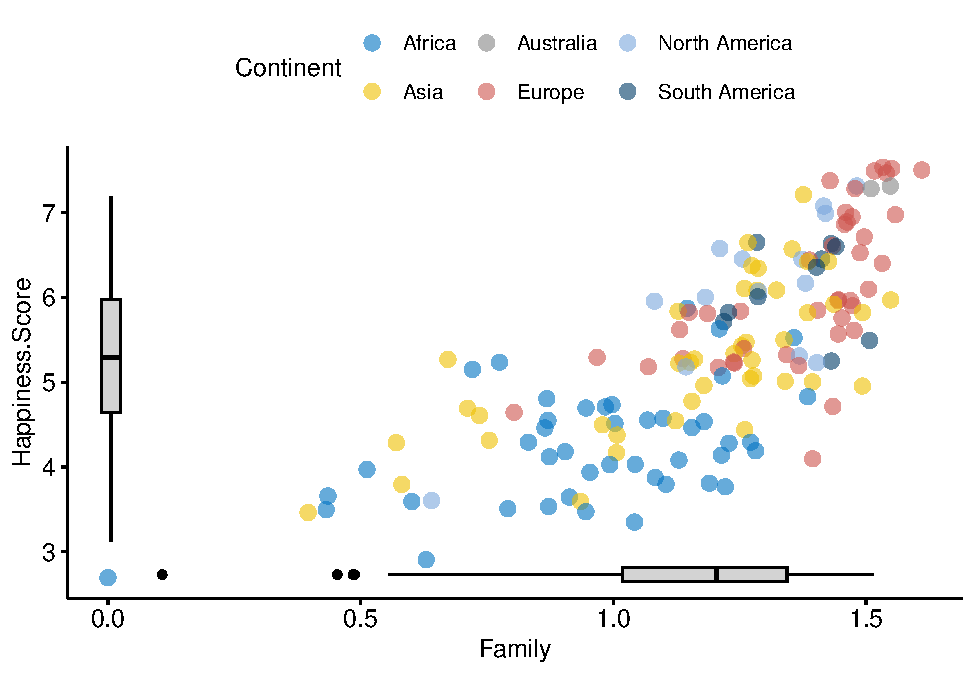
\includegraphics{Fer_files/figure-latex/unnamed-chunk-22-1.pdf}

\begin{Shaded}
\begin{Highlighting}[]
\CommentTok{\#::::::::::::::::::::::::::::Life.Expectancy::::::::::::::::::::::::::::::}
\NormalTok{sp }\OtherTok{\textless{}{-}} \FunctionTok{ggscatter}\NormalTok{(Happiness, }\AttributeTok{x =} \StringTok{"Life.Expectancy"}\NormalTok{, }\AttributeTok{y =} \StringTok{"Happiness.Score"}\NormalTok{,}
                \AttributeTok{color =} \StringTok{"Continent"}\NormalTok{, }\AttributeTok{palette =} \StringTok{"jco"}\NormalTok{,}
                \AttributeTok{size =} \DecValTok{3}\NormalTok{, }\AttributeTok{alpha =} \FloatTok{0.6}\NormalTok{)}
\CommentTok{\# Create box plots of x/y variables}
\CommentTok{\# Box plot of the x variable}
\NormalTok{xbp }\OtherTok{\textless{}{-}} \FunctionTok{ggboxplot}\NormalTok{(Happiness}\SpecialCharTok{$}\NormalTok{Life.Expectancy, }\AttributeTok{width =} \FloatTok{0.3}\NormalTok{, }\AttributeTok{fill =} \StringTok{"lightgray"}\NormalTok{) }\SpecialCharTok{+}
  \FunctionTok{rotate}\NormalTok{() }\SpecialCharTok{+}
  \FunctionTok{theme\_transparent}\NormalTok{()}
\CommentTok{\# Box plot of the y variable}
\NormalTok{ybp }\OtherTok{\textless{}{-}} \FunctionTok{ggboxplot}\NormalTok{(Happiness}\SpecialCharTok{$}\NormalTok{Happiness.Score, }\AttributeTok{width =} \FloatTok{0.3}\NormalTok{, }\AttributeTok{fill =} \StringTok{"lightgray"}\NormalTok{) }\SpecialCharTok{+}
  \FunctionTok{theme\_transparent}\NormalTok{()}
\CommentTok{\# Create the external graphical objects}
\CommentTok{\# called a "grop" in Grid terminology}
\NormalTok{xbp\_grob }\OtherTok{\textless{}{-}} \FunctionTok{ggplotGrob}\NormalTok{(xbp)}
\NormalTok{ybp\_grob }\OtherTok{\textless{}{-}} \FunctionTok{ggplotGrob}\NormalTok{(ybp)}
\CommentTok{\# Place box plots inside the scatter plot}
\NormalTok{xmin }\OtherTok{\textless{}{-}} \FunctionTok{min}\NormalTok{(Happiness}\SpecialCharTok{$}\NormalTok{Life.Expectancy); xmax }\OtherTok{\textless{}{-}} \FunctionTok{max}\NormalTok{(Happiness}\SpecialCharTok{$}\NormalTok{Life.Expectancy)}
\NormalTok{ymin }\OtherTok{\textless{}{-}} \FunctionTok{min}\NormalTok{(Happiness}\SpecialCharTok{$}\NormalTok{Happiness.Score); ymax }\OtherTok{\textless{}{-}} \FunctionTok{max}\NormalTok{(Happiness}\SpecialCharTok{$}\NormalTok{Happiness.Score)}
\NormalTok{yoffset }\OtherTok{\textless{}{-}}\NormalTok{ (}\DecValTok{1}\SpecialCharTok{/}\DecValTok{15}\NormalTok{)}\SpecialCharTok{*}\NormalTok{ymax; xoffset }\OtherTok{\textless{}{-}}\NormalTok{ (}\DecValTok{1}\SpecialCharTok{/}\DecValTok{15}\NormalTok{)}\SpecialCharTok{*}\NormalTok{xmax}
\CommentTok{\# Insert xbp\_grob inside the scatter plot}
\NormalTok{sp }\SpecialCharTok{+} \FunctionTok{annotation\_custom}\NormalTok{(}\AttributeTok{grob =}\NormalTok{ xbp\_grob, }\AttributeTok{xmin =}\NormalTok{ xmin, }\AttributeTok{xmax =}\NormalTok{ xmax, }
                       \AttributeTok{ymin =}\NormalTok{ ymin}\SpecialCharTok{{-}}\NormalTok{yoffset, }\AttributeTok{ymax =}\NormalTok{ ymin}\SpecialCharTok{+}\NormalTok{yoffset) }\SpecialCharTok{+}
  \CommentTok{\# Insert ybp\_grob inside the scatter plot}
  \FunctionTok{annotation\_custom}\NormalTok{(}\AttributeTok{grob =}\NormalTok{ ybp\_grob,}
                    \AttributeTok{xmin =}\NormalTok{ xmin}\SpecialCharTok{{-}}\NormalTok{xoffset, }\AttributeTok{xmax =}\NormalTok{ xmin}\SpecialCharTok{+}\NormalTok{xoffset, }
                    \AttributeTok{ymin =}\NormalTok{ ymin, }\AttributeTok{ymax =}\NormalTok{ ymax)}
\end{Highlighting}
\end{Shaded}

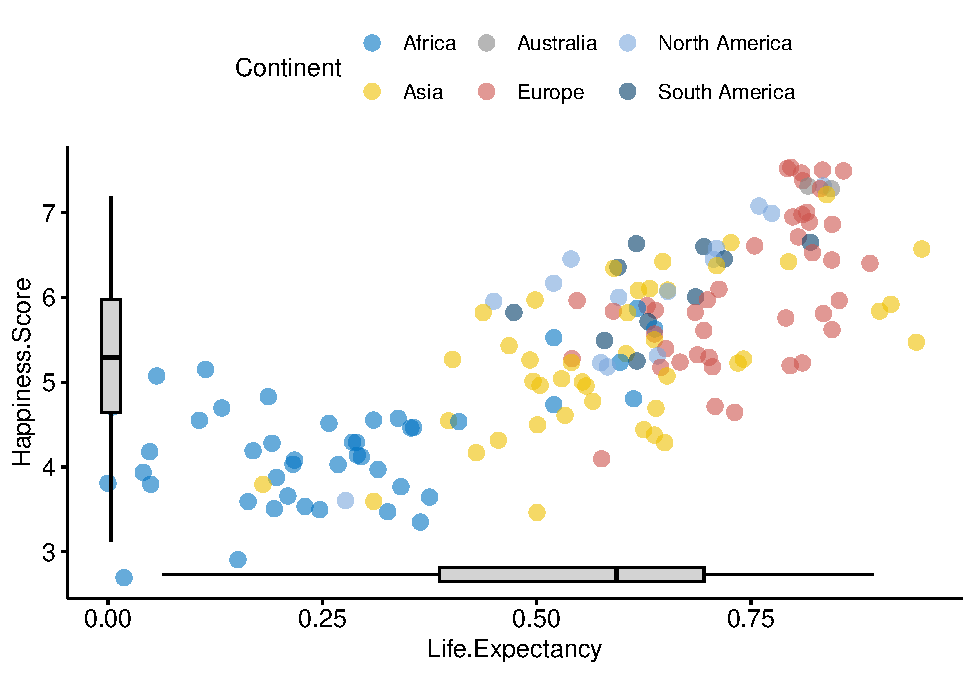
\includegraphics{Fer_files/figure-latex/unnamed-chunk-23-1.pdf}

\begin{Shaded}
\begin{Highlighting}[]
\CommentTok{\#::::::::::::::::::::::::::::Freedom::::::::::::::::::::::::::::::}
\NormalTok{sp }\OtherTok{\textless{}{-}} \FunctionTok{ggscatter}\NormalTok{(Happiness, }\AttributeTok{x =} \StringTok{"Freedom"}\NormalTok{, }\AttributeTok{y =} \StringTok{"Happiness.Score"}\NormalTok{,}
                \AttributeTok{color =} \StringTok{"Continent"}\NormalTok{, }\AttributeTok{palette =} \StringTok{"jco"}\NormalTok{,}
                \AttributeTok{size =} \DecValTok{3}\NormalTok{, }\AttributeTok{alpha =} \FloatTok{0.6}\NormalTok{)}
\CommentTok{\# Create box plots of x/y variables}
\CommentTok{\# Box plot of the x variable}
\NormalTok{xbp }\OtherTok{\textless{}{-}} \FunctionTok{ggboxplot}\NormalTok{(Happiness}\SpecialCharTok{$}\NormalTok{Freedom, }\AttributeTok{width =} \FloatTok{0.3}\NormalTok{, }\AttributeTok{fill =} \StringTok{"lightgray"}\NormalTok{) }\SpecialCharTok{+}
  \FunctionTok{rotate}\NormalTok{() }\SpecialCharTok{+}
  \FunctionTok{theme\_transparent}\NormalTok{()}
\CommentTok{\# Box plot of the y variable}
\NormalTok{ybp }\OtherTok{\textless{}{-}} \FunctionTok{ggboxplot}\NormalTok{(Happiness}\SpecialCharTok{$}\NormalTok{Happiness.Score, }\AttributeTok{width =} \FloatTok{0.3}\NormalTok{, }\AttributeTok{fill =} \StringTok{"lightgray"}\NormalTok{) }\SpecialCharTok{+}
  \FunctionTok{theme\_transparent}\NormalTok{()}
\CommentTok{\# Create the external graphical objects}
\CommentTok{\# called a "grop" in Grid terminology}
\NormalTok{xbp\_grob }\OtherTok{\textless{}{-}} \FunctionTok{ggplotGrob}\NormalTok{(xbp)}
\NormalTok{ybp\_grob }\OtherTok{\textless{}{-}} \FunctionTok{ggplotGrob}\NormalTok{(ybp)}
\CommentTok{\# Place box plots inside the scatter plot}
\NormalTok{xmin }\OtherTok{\textless{}{-}} \FunctionTok{min}\NormalTok{(Happiness}\SpecialCharTok{$}\NormalTok{Freedom); xmax }\OtherTok{\textless{}{-}} \FunctionTok{max}\NormalTok{(Happiness}\SpecialCharTok{$}\NormalTok{Freedom)}
\NormalTok{ymin }\OtherTok{\textless{}{-}} \FunctionTok{min}\NormalTok{(Happiness}\SpecialCharTok{$}\NormalTok{Happiness.Score); ymax }\OtherTok{\textless{}{-}} \FunctionTok{max}\NormalTok{(Happiness}\SpecialCharTok{$}\NormalTok{Happiness.Score)}
\NormalTok{yoffset }\OtherTok{\textless{}{-}}\NormalTok{ (}\DecValTok{1}\SpecialCharTok{/}\DecValTok{15}\NormalTok{)}\SpecialCharTok{*}\NormalTok{ymax; xoffset }\OtherTok{\textless{}{-}}\NormalTok{ (}\DecValTok{1}\SpecialCharTok{/}\DecValTok{15}\NormalTok{)}\SpecialCharTok{*}\NormalTok{xmax}
\CommentTok{\# Insert xbp\_grob inside the scatter plot}
\NormalTok{sp }\SpecialCharTok{+} \FunctionTok{annotation\_custom}\NormalTok{(}\AttributeTok{grob =}\NormalTok{ xbp\_grob, }\AttributeTok{xmin =}\NormalTok{ xmin, }\AttributeTok{xmax =}\NormalTok{ xmax, }
                       \AttributeTok{ymin =}\NormalTok{ ymin}\SpecialCharTok{{-}}\NormalTok{yoffset, }\AttributeTok{ymax =}\NormalTok{ ymin}\SpecialCharTok{+}\NormalTok{yoffset) }\SpecialCharTok{+}
  \CommentTok{\# Insert ybp\_grob inside the scatter plot}
  \FunctionTok{annotation\_custom}\NormalTok{(}\AttributeTok{grob =}\NormalTok{ ybp\_grob,}
                    \AttributeTok{xmin =}\NormalTok{ xmin}\SpecialCharTok{{-}}\NormalTok{xoffset, }\AttributeTok{xmax =}\NormalTok{ xmin}\SpecialCharTok{+}\NormalTok{xoffset, }
                    \AttributeTok{ymin =}\NormalTok{ ymin, }\AttributeTok{ymax =}\NormalTok{ ymax)}
\end{Highlighting}
\end{Shaded}

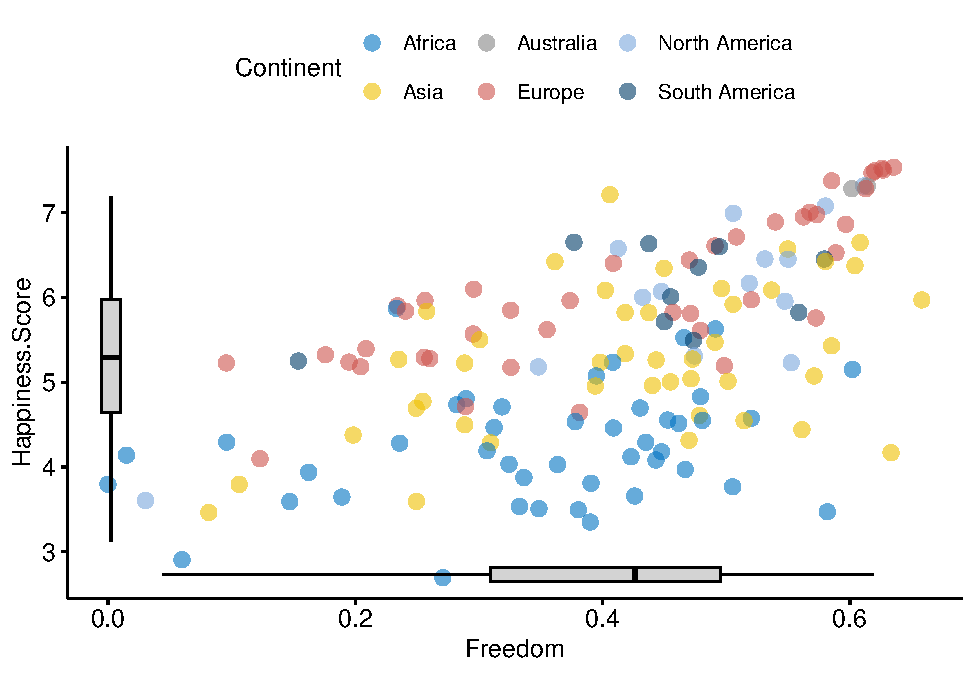
\includegraphics{Fer_files/figure-latex/unnamed-chunk-24-1.pdf}

\begin{Shaded}
\begin{Highlighting}[]
\CommentTok{\#::::::::::::::::::::::::::::Economy::::::::::::::::::::::::::::::}
\NormalTok{sp }\OtherTok{\textless{}{-}} \FunctionTok{ggscatter}\NormalTok{(Happiness, }\AttributeTok{x =} \StringTok{"Economy"}\NormalTok{, }\AttributeTok{y =} \StringTok{"Happiness.Score"}\NormalTok{,}
                \AttributeTok{color =} \StringTok{"Continent"}\NormalTok{, }\AttributeTok{palette =} \StringTok{"jco"}\NormalTok{,}
                \AttributeTok{size =} \DecValTok{3}\NormalTok{, }\AttributeTok{alpha =} \FloatTok{0.6}\NormalTok{)}
\CommentTok{\# Create box plots of x/y variables}
\CommentTok{\# Box plot of the x variable}
\NormalTok{xbp }\OtherTok{\textless{}{-}} \FunctionTok{ggboxplot}\NormalTok{(Happiness}\SpecialCharTok{$}\NormalTok{Economy, }\AttributeTok{width =} \FloatTok{0.3}\NormalTok{, }\AttributeTok{fill =} \StringTok{"lightgray"}\NormalTok{) }\SpecialCharTok{+}
  \FunctionTok{rotate}\NormalTok{() }\SpecialCharTok{+}
  \FunctionTok{theme\_transparent}\NormalTok{()}
\CommentTok{\# Box plot of the y variable}
\NormalTok{ybp }\OtherTok{\textless{}{-}} \FunctionTok{ggboxplot}\NormalTok{(Happiness}\SpecialCharTok{$}\NormalTok{Happiness.Score, }\AttributeTok{width =} \FloatTok{0.3}\NormalTok{, }\AttributeTok{fill =} \StringTok{"lightgray"}\NormalTok{) }\SpecialCharTok{+}
  \FunctionTok{theme\_transparent}\NormalTok{()}
\CommentTok{\# Create the external graphical objects}
\CommentTok{\# called a "grop" in Grid terminology}
\NormalTok{xbp\_grob }\OtherTok{\textless{}{-}} \FunctionTok{ggplotGrob}\NormalTok{(xbp)}
\NormalTok{ybp\_grob }\OtherTok{\textless{}{-}} \FunctionTok{ggplotGrob}\NormalTok{(ybp)}
\CommentTok{\# Place box plots inside the scatter plot}
\NormalTok{xmin }\OtherTok{\textless{}{-}} \FunctionTok{min}\NormalTok{(Happiness}\SpecialCharTok{$}\NormalTok{Economy); xmax }\OtherTok{\textless{}{-}} \FunctionTok{max}\NormalTok{(Happiness}\SpecialCharTok{$}\NormalTok{Economy)}
\NormalTok{ymin }\OtherTok{\textless{}{-}} \FunctionTok{min}\NormalTok{(Happiness}\SpecialCharTok{$}\NormalTok{Happiness.Score); ymax }\OtherTok{\textless{}{-}} \FunctionTok{max}\NormalTok{(Happiness}\SpecialCharTok{$}\NormalTok{Happiness.Score)}
\NormalTok{yoffset }\OtherTok{\textless{}{-}}\NormalTok{ (}\DecValTok{1}\SpecialCharTok{/}\DecValTok{15}\NormalTok{)}\SpecialCharTok{*}\NormalTok{ymax; xoffset }\OtherTok{\textless{}{-}}\NormalTok{ (}\DecValTok{1}\SpecialCharTok{/}\DecValTok{15}\NormalTok{)}\SpecialCharTok{*}\NormalTok{xmax}
\CommentTok{\# Insert xbp\_grob inside the scatter plot}
\NormalTok{sp }\SpecialCharTok{+} \FunctionTok{annotation\_custom}\NormalTok{(}\AttributeTok{grob =}\NormalTok{ xbp\_grob, }\AttributeTok{xmin =}\NormalTok{ xmin, }\AttributeTok{xmax =}\NormalTok{ xmax, }
                       \AttributeTok{ymin =}\NormalTok{ ymin}\SpecialCharTok{{-}}\NormalTok{yoffset, }\AttributeTok{ymax =}\NormalTok{ ymin}\SpecialCharTok{+}\NormalTok{yoffset) }\SpecialCharTok{+}
  \CommentTok{\# Insert ybp\_grob inside the scatter plot}
  \FunctionTok{annotation\_custom}\NormalTok{(}\AttributeTok{grob =}\NormalTok{ ybp\_grob,}
                    \AttributeTok{xmin =}\NormalTok{ xmin}\SpecialCharTok{{-}}\NormalTok{xoffset, }\AttributeTok{xmax =}\NormalTok{ xmin}\SpecialCharTok{+}\NormalTok{xoffset, }
                    \AttributeTok{ymin =}\NormalTok{ ymin, }\AttributeTok{ymax =}\NormalTok{ ymax)}
\end{Highlighting}
\end{Shaded}

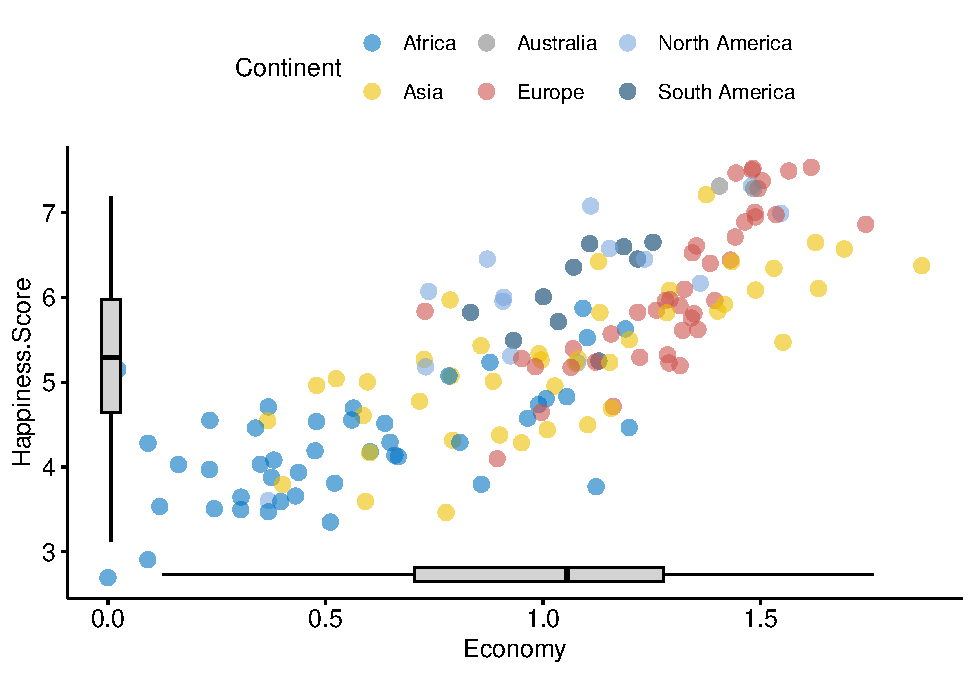
\includegraphics{Fer_files/figure-latex/unnamed-chunk-25-1.pdf}

\begin{Shaded}
\begin{Highlighting}[]
\CommentTok{\#::::::::::::::::::::::::::::Trust::::::::::::::::::::::::::::::}
\NormalTok{sp }\OtherTok{\textless{}{-}} \FunctionTok{ggscatter}\NormalTok{(Happiness, }\AttributeTok{x =} \StringTok{"Trust"}\NormalTok{, }\AttributeTok{y =} \StringTok{"Happiness.Score"}\NormalTok{,}
                \AttributeTok{color =} \StringTok{"Continent"}\NormalTok{, }\AttributeTok{palette =} \StringTok{"jco"}\NormalTok{,}
                \AttributeTok{size =} \DecValTok{3}\NormalTok{, }\AttributeTok{alpha =} \FloatTok{0.6}\NormalTok{)}
\CommentTok{\# Create box plots of x/y variables}
\CommentTok{\# Box plot of the x variable}
\NormalTok{xbp }\OtherTok{\textless{}{-}} \FunctionTok{ggboxplot}\NormalTok{(Happiness}\SpecialCharTok{$}\NormalTok{Trust, }\AttributeTok{width =} \FloatTok{0.3}\NormalTok{, }\AttributeTok{fill =} \StringTok{"lightgray"}\NormalTok{) }\SpecialCharTok{+}
  \FunctionTok{rotate}\NormalTok{() }\SpecialCharTok{+}
  \FunctionTok{theme\_transparent}\NormalTok{()}
\CommentTok{\# Box plot of the y variable}
\NormalTok{ybp }\OtherTok{\textless{}{-}} \FunctionTok{ggboxplot}\NormalTok{(Happiness}\SpecialCharTok{$}\NormalTok{Happiness.Score, }\AttributeTok{width =} \FloatTok{0.3}\NormalTok{, }\AttributeTok{fill =} \StringTok{"lightgray"}\NormalTok{) }\SpecialCharTok{+}
  \FunctionTok{theme\_transparent}\NormalTok{()}
\CommentTok{\# Create the external graphical objects}
\CommentTok{\# called a "grop" in Grid terminology}
\NormalTok{xbp\_grob }\OtherTok{\textless{}{-}} \FunctionTok{ggplotGrob}\NormalTok{(xbp)}
\NormalTok{ybp\_grob }\OtherTok{\textless{}{-}} \FunctionTok{ggplotGrob}\NormalTok{(ybp)}
\CommentTok{\# Place box plots inside the scatter plot}
\NormalTok{xmin }\OtherTok{\textless{}{-}} \FunctionTok{min}\NormalTok{(Happiness}\SpecialCharTok{$}\NormalTok{Trust); xmax }\OtherTok{\textless{}{-}} \FunctionTok{max}\NormalTok{(Happiness}\SpecialCharTok{$}\NormalTok{Trust)}
\NormalTok{ymin }\OtherTok{\textless{}{-}} \FunctionTok{min}\NormalTok{(Happiness}\SpecialCharTok{$}\NormalTok{Happiness.Score); ymax }\OtherTok{\textless{}{-}} \FunctionTok{max}\NormalTok{(Happiness}\SpecialCharTok{$}\NormalTok{Happiness.Score)}
\NormalTok{yoffset }\OtherTok{\textless{}{-}}\NormalTok{ (}\DecValTok{1}\SpecialCharTok{/}\DecValTok{15}\NormalTok{)}\SpecialCharTok{*}\NormalTok{ymax; xoffset }\OtherTok{\textless{}{-}}\NormalTok{ (}\DecValTok{1}\SpecialCharTok{/}\DecValTok{15}\NormalTok{)}\SpecialCharTok{*}\NormalTok{xmax}
\CommentTok{\# Insert xbp\_grob inside the scatter plot}
\NormalTok{sp }\SpecialCharTok{+} \FunctionTok{annotation\_custom}\NormalTok{(}\AttributeTok{grob =}\NormalTok{ xbp\_grob, }\AttributeTok{xmin =}\NormalTok{ xmin, }\AttributeTok{xmax =}\NormalTok{ xmax, }
                       \AttributeTok{ymin =}\NormalTok{ ymin}\SpecialCharTok{{-}}\NormalTok{yoffset, }\AttributeTok{ymax =}\NormalTok{ ymin}\SpecialCharTok{+}\NormalTok{yoffset) }\SpecialCharTok{+}
  \CommentTok{\# Insert ybp\_grob inside the scatter plot}
  \FunctionTok{annotation\_custom}\NormalTok{(}\AttributeTok{grob =}\NormalTok{ ybp\_grob,}
                    \AttributeTok{xmin =}\NormalTok{ xmin}\SpecialCharTok{{-}}\NormalTok{xoffset, }\AttributeTok{xmax =}\NormalTok{ xmin}\SpecialCharTok{+}\NormalTok{xoffset, }
                    \AttributeTok{ymin =}\NormalTok{ ymin, }\AttributeTok{ymax =}\NormalTok{ ymax)}
\end{Highlighting}
\end{Shaded}

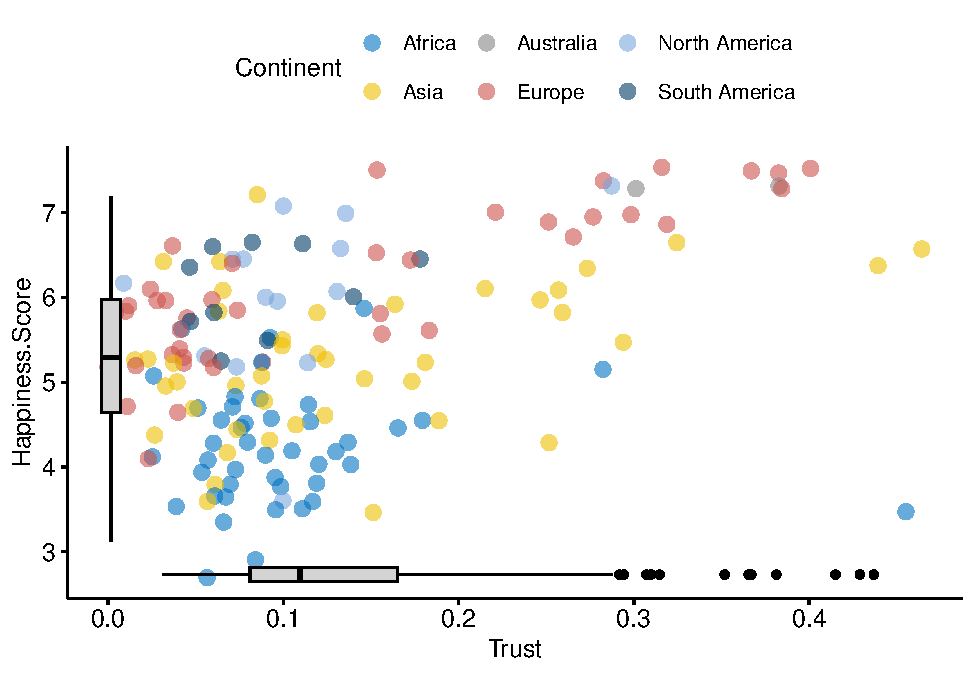
\includegraphics{Fer_files/figure-latex/unnamed-chunk-26-1.pdf}

\begin{Shaded}
\begin{Highlighting}[]
\CommentTok{\#::::::::::::::::::::::::::::Dystopia.Residual::::::::::::::::::::::::::::::}
\NormalTok{sp }\OtherTok{\textless{}{-}} \FunctionTok{ggscatter}\NormalTok{(Happiness, }\AttributeTok{x =} \StringTok{"Dystopia.Residual"}\NormalTok{, }\AttributeTok{y =} \StringTok{"Happiness.Score"}\NormalTok{,}
                \AttributeTok{color =} \StringTok{"Continent"}\NormalTok{, }\AttributeTok{palette =} \StringTok{"jco"}\NormalTok{,}
                \AttributeTok{size =} \DecValTok{3}\NormalTok{, }\AttributeTok{alpha =} \FloatTok{0.6}\NormalTok{)}
\CommentTok{\# Create box plots of x/y variables}
\CommentTok{\# Box plot of the x variable}
\NormalTok{xbp }\OtherTok{\textless{}{-}} \FunctionTok{ggboxplot}\NormalTok{(Happiness}\SpecialCharTok{$}\NormalTok{Dystopia.Residual, }\AttributeTok{width =} \FloatTok{0.3}\NormalTok{, }\AttributeTok{fill =} \StringTok{"lightgray"}\NormalTok{) }\SpecialCharTok{+}
  \FunctionTok{rotate}\NormalTok{() }\SpecialCharTok{+}
  \FunctionTok{theme\_transparent}\NormalTok{()}
\CommentTok{\# Box plot of the y variable}
\NormalTok{ybp }\OtherTok{\textless{}{-}} \FunctionTok{ggboxplot}\NormalTok{(Happiness}\SpecialCharTok{$}\NormalTok{Happiness.Score, }\AttributeTok{width =} \FloatTok{0.3}\NormalTok{, }\AttributeTok{fill =} \StringTok{"lightgray"}\NormalTok{) }\SpecialCharTok{+}
  \FunctionTok{theme\_transparent}\NormalTok{()}
\CommentTok{\# Create the external graphical objects}
\CommentTok{\# called a "grop" in Grid terminology}
\NormalTok{xbp\_grob }\OtherTok{\textless{}{-}} \FunctionTok{ggplotGrob}\NormalTok{(xbp)}
\NormalTok{ybp\_grob }\OtherTok{\textless{}{-}} \FunctionTok{ggplotGrob}\NormalTok{(ybp)}
\CommentTok{\# Place box plots inside the scatter plot}
\NormalTok{xmin }\OtherTok{\textless{}{-}} \FunctionTok{min}\NormalTok{(Happiness}\SpecialCharTok{$}\NormalTok{Dystopia.Residual); xmax }\OtherTok{\textless{}{-}} \FunctionTok{max}\NormalTok{(Happiness}\SpecialCharTok{$}\NormalTok{Dystopia.Residual)}
\NormalTok{ymin }\OtherTok{\textless{}{-}} \FunctionTok{min}\NormalTok{(Happiness}\SpecialCharTok{$}\NormalTok{Happiness.Score); ymax }\OtherTok{\textless{}{-}} \FunctionTok{max}\NormalTok{(Happiness}\SpecialCharTok{$}\NormalTok{Happiness.Score)}
\NormalTok{yoffset }\OtherTok{\textless{}{-}}\NormalTok{ (}\DecValTok{1}\SpecialCharTok{/}\DecValTok{15}\NormalTok{)}\SpecialCharTok{*}\NormalTok{ymax; xoffset }\OtherTok{\textless{}{-}}\NormalTok{ (}\DecValTok{1}\SpecialCharTok{/}\DecValTok{15}\NormalTok{)}\SpecialCharTok{*}\NormalTok{xmax}
\CommentTok{\# Insert xbp\_grob inside the scatter plot}
\NormalTok{sp }\SpecialCharTok{+} \FunctionTok{annotation\_custom}\NormalTok{(}\AttributeTok{grob =}\NormalTok{ xbp\_grob, }\AttributeTok{xmin =}\NormalTok{ xmin, }\AttributeTok{xmax =}\NormalTok{ xmax, }
                       \AttributeTok{ymin =}\NormalTok{ ymin}\SpecialCharTok{{-}}\NormalTok{yoffset, }\AttributeTok{ymax =}\NormalTok{ ymin}\SpecialCharTok{+}\NormalTok{yoffset) }\SpecialCharTok{+}
  \CommentTok{\# Insert ybp\_grob inside the scatter plot}
  \FunctionTok{annotation\_custom}\NormalTok{(}\AttributeTok{grob =}\NormalTok{ ybp\_grob,}
                    \AttributeTok{xmin =}\NormalTok{ xmin}\SpecialCharTok{{-}}\NormalTok{xoffset, }\AttributeTok{xmax =}\NormalTok{ xmin}\SpecialCharTok{+}\NormalTok{xoffset, }
                    \AttributeTok{ymin =}\NormalTok{ ymin, }\AttributeTok{ymax =}\NormalTok{ ymax)}
\end{Highlighting}
\end{Shaded}

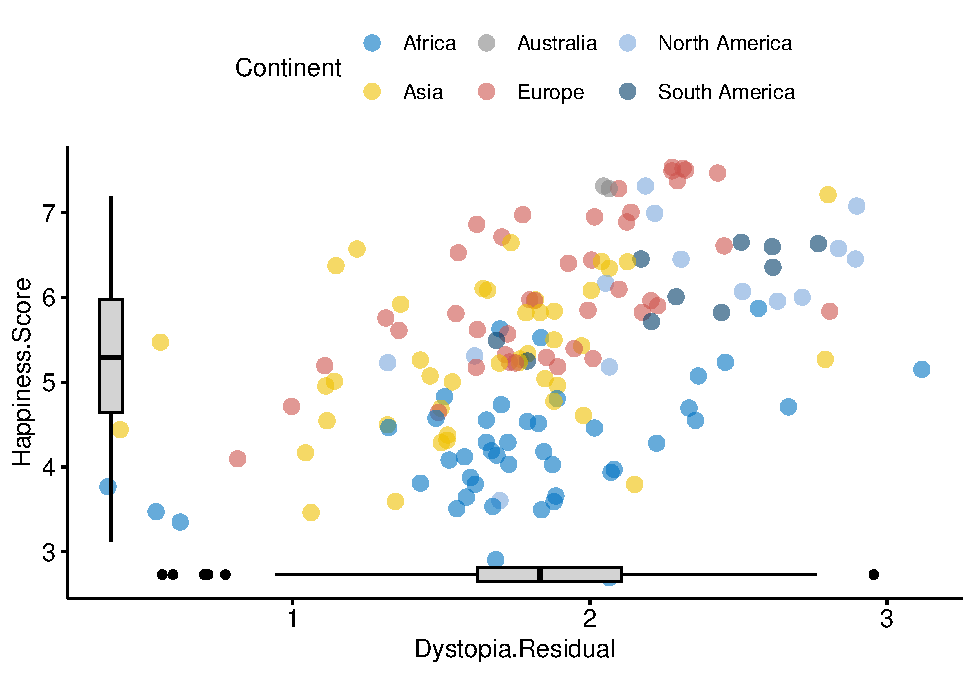
\includegraphics{Fer_files/figure-latex/unnamed-chunk-27-1.pdf}

\subsection{3D Plot}\label{d-plot}

For the last part of our visualization let's create some fancy plots. I
have to indicate that I am not in favor of 3D plots or any fancy plots
but let's do this just for fun!

\begin{Shaded}
\begin{Highlighting}[]
\FunctionTok{scatter3D}\NormalTok{(Happiness}\SpecialCharTok{$}\NormalTok{Freedom, Happiness}\SpecialCharTok{$}\NormalTok{Life.Expectancy, Happiness}\SpecialCharTok{$}\NormalTok{Happiness.Score, }\AttributeTok{phi =} \DecValTok{0}\NormalTok{, }\AttributeTok{bty =} \StringTok{"g"}\NormalTok{,}
          \AttributeTok{pch =} \DecValTok{20}\NormalTok{, }\AttributeTok{cex =} \DecValTok{2}\NormalTok{, }\AttributeTok{ticktype =} \StringTok{"detailed"}\NormalTok{,}
          \AttributeTok{main =} \StringTok{"Happiness data"}\NormalTok{, }\AttributeTok{xlab =} \StringTok{"Freedom"}\NormalTok{,}
          \AttributeTok{ylab =}\StringTok{"Life.Expectancy"}\NormalTok{, }\AttributeTok{zlab =} \StringTok{"Happiness.Score"}\NormalTok{)}
\end{Highlighting}
\end{Shaded}

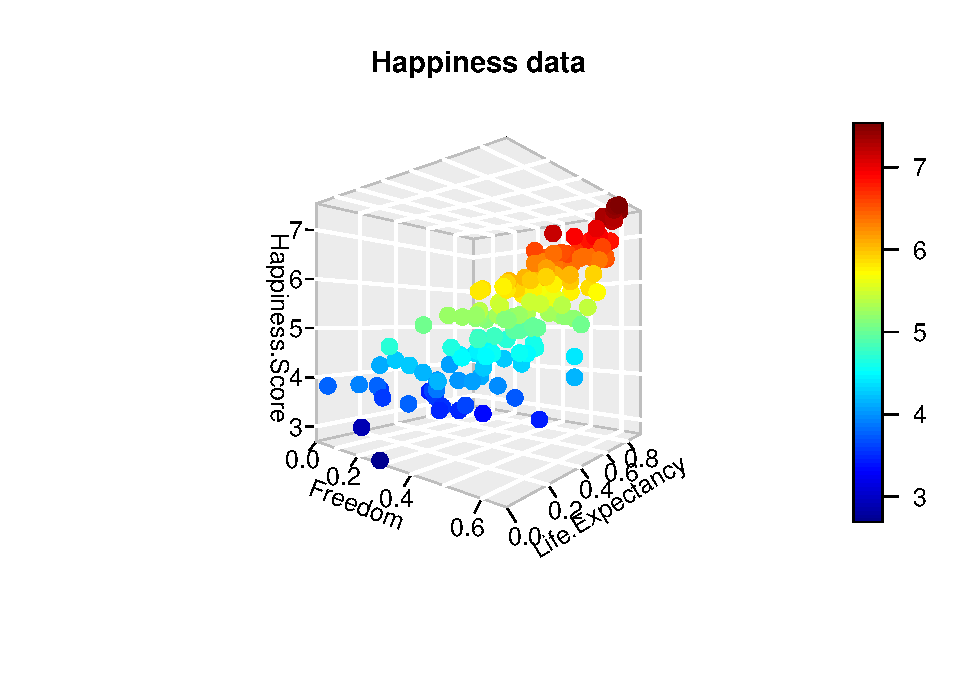
\includegraphics{Fer_files/figure-latex/unnamed-chunk-28-1.pdf}

According to this plot, the higher the life expectancy and freedom
scores, the higher will be the happiness score.

\begin{Shaded}
\begin{Highlighting}[]
\FunctionTok{scatter3D}\NormalTok{(Happiness}\SpecialCharTok{$}\NormalTok{Generosity, Happiness}\SpecialCharTok{$}\NormalTok{Economy, Happiness}\SpecialCharTok{$}\NormalTok{Happiness.Score, }\AttributeTok{phi =} \DecValTok{0}\NormalTok{, }\AttributeTok{bty =} \StringTok{"g"}\NormalTok{,}
          \AttributeTok{pch =} \DecValTok{20}\NormalTok{, }\AttributeTok{cex =} \DecValTok{2}\NormalTok{, }\AttributeTok{ticktype =} \StringTok{"detailed"}\NormalTok{,}
          \AttributeTok{main =} \StringTok{"Happiness data"}\NormalTok{, }\AttributeTok{xlab =} \StringTok{"Generosity"}\NormalTok{,}
          \AttributeTok{ylab =}\StringTok{"Economy"}\NormalTok{, }\AttributeTok{zlab =} \StringTok{"Happiness.Score"}\NormalTok{)}
\end{Highlighting}
\end{Shaded}

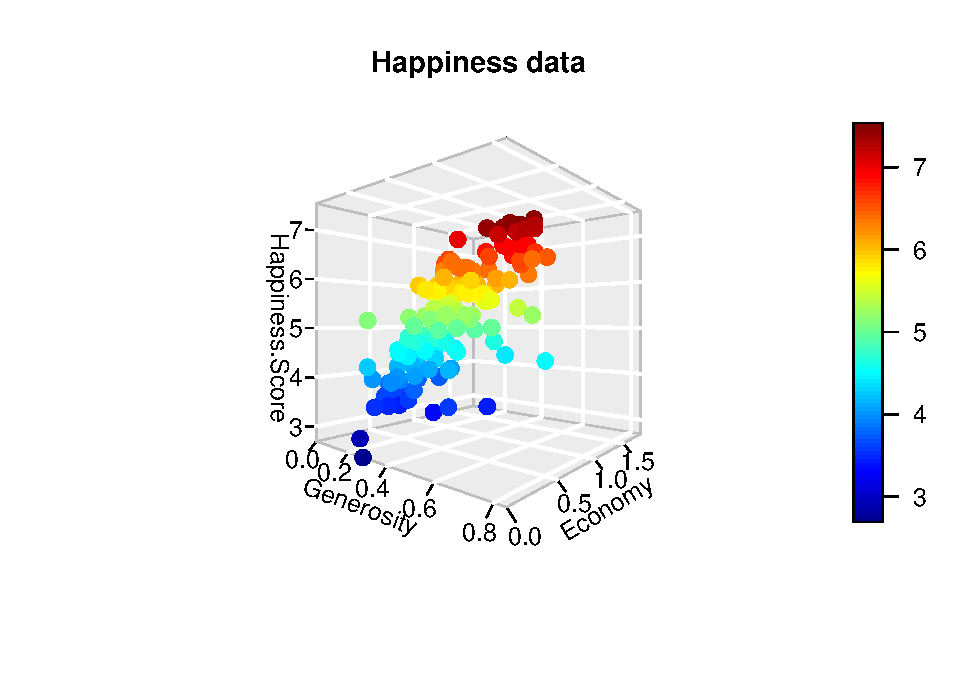
\includegraphics{Fer_files/figure-latex/unnamed-chunk-29-1.pdf}

The higher economy score and the lower generosity score will lead to the
higher level of happiness.

\begin{Shaded}
\begin{Highlighting}[]
\FunctionTok{scatter3D}\NormalTok{(Happiness}\SpecialCharTok{$}\NormalTok{Trust, Happiness}\SpecialCharTok{$}\NormalTok{Freedom, Happiness}\SpecialCharTok{$}\NormalTok{Happiness.Score, }\AttributeTok{phi =} \DecValTok{0}\NormalTok{, }\AttributeTok{bty =} \StringTok{"g"}\NormalTok{,}
          \AttributeTok{pch =} \DecValTok{20}\NormalTok{, }\AttributeTok{cex =} \DecValTok{2}\NormalTok{, }\AttributeTok{ticktype =} \StringTok{"detailed"}\NormalTok{,}
          \AttributeTok{main =} \StringTok{"Happiness data"}\NormalTok{, }\AttributeTok{xlab =} \StringTok{"Trust"}\NormalTok{,}
          \AttributeTok{ylab =}\StringTok{"Freedom"}\NormalTok{, }\AttributeTok{zlab =} \StringTok{"Happiness.Score"}\NormalTok{)}
\end{Highlighting}
\end{Shaded}

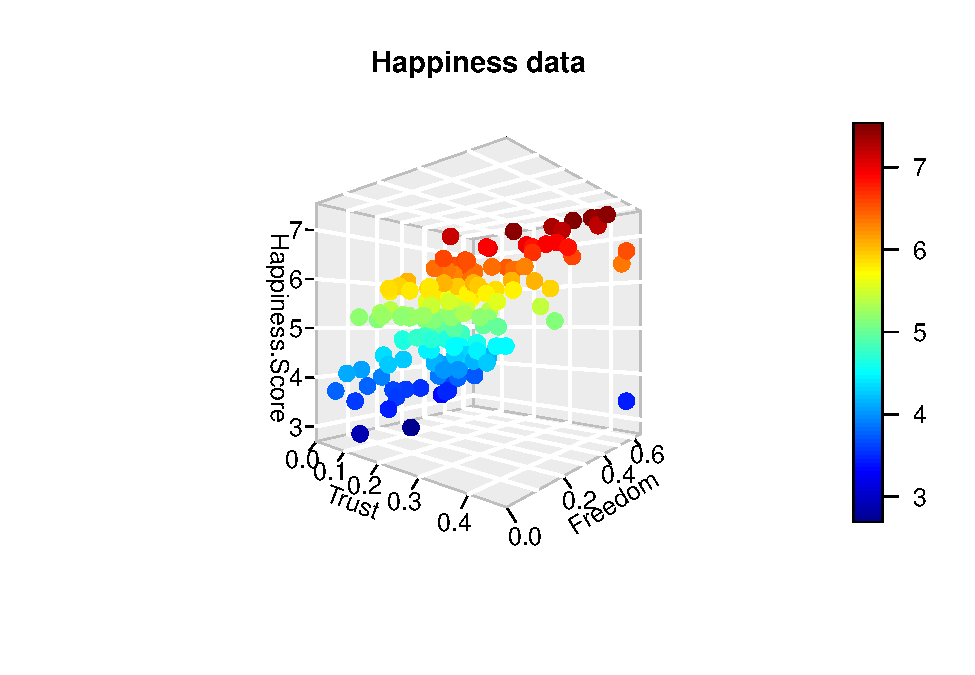
\includegraphics{Fer_files/figure-latex/unnamed-chunk-30-1.pdf}

In general, trust is not a significant factor to have a higher happiness
score, but we can see that for the countries which freedom is a
significant factor, and the happiness score is more than 7, trust plays
a significant role.

\begin{Shaded}
\begin{Highlighting}[]
\FunctionTok{scatter3D}\NormalTok{(Happiness}\SpecialCharTok{$}\NormalTok{Family, Happiness}\SpecialCharTok{$}\NormalTok{Economy, Happiness}\SpecialCharTok{$}\NormalTok{Happiness.Score, }\AttributeTok{phi =} \DecValTok{0}\NormalTok{, }\AttributeTok{bty =} \StringTok{"g"}\NormalTok{,}
          \AttributeTok{pch =} \DecValTok{20}\NormalTok{, }\AttributeTok{cex =} \DecValTok{2}\NormalTok{, }\AttributeTok{ticktype =} \StringTok{"detailed"}\NormalTok{,}
          \AttributeTok{main =} \StringTok{"Happiness data"}\NormalTok{, }\AttributeTok{xlab =} \StringTok{"Trust"}\NormalTok{,}
          \AttributeTok{ylab =}\StringTok{"Economy"}\NormalTok{, }\AttributeTok{zlab =} \StringTok{"Happiness.Score"}\NormalTok{)}
\end{Highlighting}
\end{Shaded}

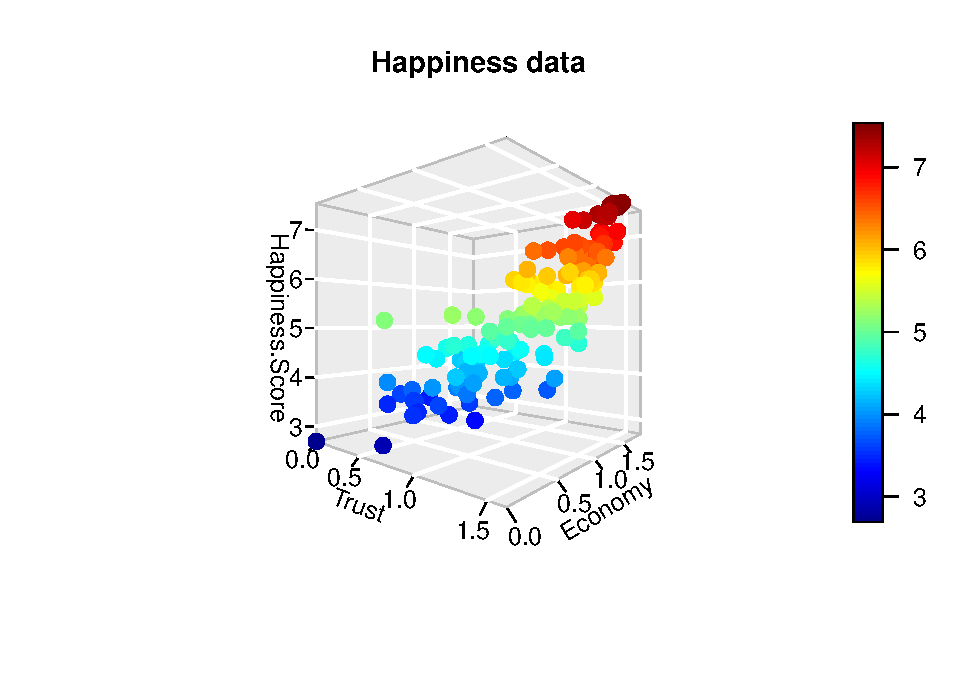
\includegraphics{Fer_files/figure-latex/unnamed-chunk-31-1.pdf}

With an increase in the economy score and the happiness score, trust
remains constant. This is the trend for happiness scores below 5. After
this point, we can see that the impact of trust on happiness score
increases gradually.

\section{Prediction}\label{prediction}

In this section, we will implement several machine learning algorithms
to predict happiness score. First, we should split our dataset into
training and test set. Our dependent variable is happiness score, and
the independent variables are family, economy, life expectancy, trust,
freedom, generosity, and dystopia residual.

\begin{Shaded}
\begin{Highlighting}[]
\CommentTok{\# Splitting the dataset into the Training set and Test set}
\CommentTok{\# install.packages(\textquotesingle{}caTools\textquotesingle{})}
\FunctionTok{library}\NormalTok{(caTools)}
\FunctionTok{set.seed}\NormalTok{(}\DecValTok{123}\NormalTok{)}
\NormalTok{dataset }\OtherTok{\textless{}{-}}\NormalTok{ Happiness[}\DecValTok{4}\SpecialCharTok{:}\DecValTok{11}\NormalTok{]}
\NormalTok{split }\OtherTok{=} \FunctionTok{sample.split}\NormalTok{(dataset}\SpecialCharTok{$}\NormalTok{Happiness.Score, }\AttributeTok{SplitRatio =} \FloatTok{0.8}\NormalTok{)}
\NormalTok{training\_set }\OtherTok{=} \FunctionTok{subset}\NormalTok{(dataset, split }\SpecialCharTok{==} \ConstantTok{TRUE}\NormalTok{)}
\NormalTok{test\_set }\OtherTok{=} \FunctionTok{subset}\NormalTok{(dataset, split }\SpecialCharTok{==} \ConstantTok{FALSE}\NormalTok{)}
\end{Highlighting}
\end{Shaded}

\textbf{Multiple Linear Regression}

\begin{Shaded}
\begin{Highlighting}[]
\CommentTok{\# Fitting Multiple Linear Regression to the Training set}
\NormalTok{regressor\_lm }\OtherTok{=} \FunctionTok{lm}\NormalTok{(}\AttributeTok{formula =}\NormalTok{ Happiness.Score }\SpecialCharTok{\textasciitilde{}}\NormalTok{ .,}
               \AttributeTok{data =}\NormalTok{ training\_set)}

\FunctionTok{summary}\NormalTok{(regressor\_lm)}
\end{Highlighting}
\end{Shaded}

\begin{verbatim}
## 
## Call:
## lm(formula = Happiness.Score ~ ., data = training_set)
## 
## Residuals:
##        Min         1Q     Median         3Q        Max 
## -5.907e-04 -2.008e-04 -1.600e-07  2.510e-04  4.855e-04 
## 
## Coefficients:
##                    Estimate Std. Error   t value Pr(>|t|)    
## (Intercept)       1.701e-04  1.509e-04     1.127    0.262    
## Economy           1.000e+00  1.300e-04  7690.839   <2e-16 ***
## Family            9.999e-01  1.253e-04  7981.804   <2e-16 ***
## Life.Expectancy   9.997e-01  2.122e-04  4711.655   <2e-16 ***
## Freedom           9.999e-01  2.245e-04  4453.253   <2e-16 ***
## Generosity        1.000e+00  2.310e-04  4330.040   <2e-16 ***
## Trust             9.997e-01  3.335e-04  2997.191   <2e-16 ***
## Dystopia.Residual 1.000e+00  5.452e-05 18343.021   <2e-16 ***
## ---
## Signif. codes:  0 '***' 0.001 '**' 0.01 '*' 0.05 '.' 0.1 ' ' 1
## 
## Residual standard error: 0.0002848 on 116 degrees of freedom
## Multiple R-squared:      1,  Adjusted R-squared:      1 
## F-statistic: 2.689e+08 on 7 and 116 DF,  p-value: < 2.2e-16
\end{verbatim}

The summary shows that all independent variables have a significant
impact, and adjusted R squared is 1! As we discussed, it is clear that
there is a linear correlation between dependent and independent
variables. Again, I should mention that the sum of the independent
variables is equal to the dependent variable which is the happiness
score. This is the justification for having an adjusted R squared equals
to 1. As a result, I guess Multiple Linear Regression will predict
happiness scores with 100 \% accuracy!

\begin{Shaded}
\begin{Highlighting}[]
\DocumentationTok{\#\#\#\#\#\#\# Predicting the Test set results}
\NormalTok{y\_pred\_lm }\OtherTok{=} \FunctionTok{predict}\NormalTok{(regressor\_lm, }\AttributeTok{newdata =}\NormalTok{ test\_set)}

\NormalTok{Pred\_Actual\_lm }\OtherTok{\textless{}{-}} \FunctionTok{as.data.frame}\NormalTok{(}\FunctionTok{cbind}\NormalTok{(}\AttributeTok{Prediction =}\NormalTok{ y\_pred\_lm, }\AttributeTok{Actual =}\NormalTok{ test\_set}\SpecialCharTok{$}\NormalTok{Happiness.Score))}

\NormalTok{gg.lm }\OtherTok{\textless{}{-}} \FunctionTok{ggplot}\NormalTok{(Pred\_Actual\_lm, }\FunctionTok{aes}\NormalTok{(Actual, Prediction )) }\SpecialCharTok{+}
  \FunctionTok{geom\_point}\NormalTok{() }\SpecialCharTok{+} \FunctionTok{theme\_bw}\NormalTok{() }\SpecialCharTok{+} \FunctionTok{geom\_abline}\NormalTok{() }\SpecialCharTok{+}
  \FunctionTok{labs}\NormalTok{(}\AttributeTok{title =} \StringTok{"Multiple Linear Regression"}\NormalTok{, }\AttributeTok{x =} \StringTok{"Actual happiness score"}\NormalTok{,}
       \AttributeTok{y =} \StringTok{"Predicted happiness score"}\NormalTok{) }\SpecialCharTok{+}
  \FunctionTok{theme}\NormalTok{(}\AttributeTok{plot.title =} \FunctionTok{element\_text}\NormalTok{(}\AttributeTok{family =} \StringTok{"Helvetica"}\NormalTok{, }\AttributeTok{face =} \StringTok{"bold"}\NormalTok{, }\AttributeTok{size =}\NormalTok{ (}\DecValTok{15}\NormalTok{)), }
        \AttributeTok{axis.title =} \FunctionTok{element\_text}\NormalTok{(}\AttributeTok{family =} \StringTok{"Helvetica"}\NormalTok{, }\AttributeTok{size =}\NormalTok{ (}\DecValTok{10}\NormalTok{)))}
\NormalTok{gg.lm}
\end{Highlighting}
\end{Shaded}

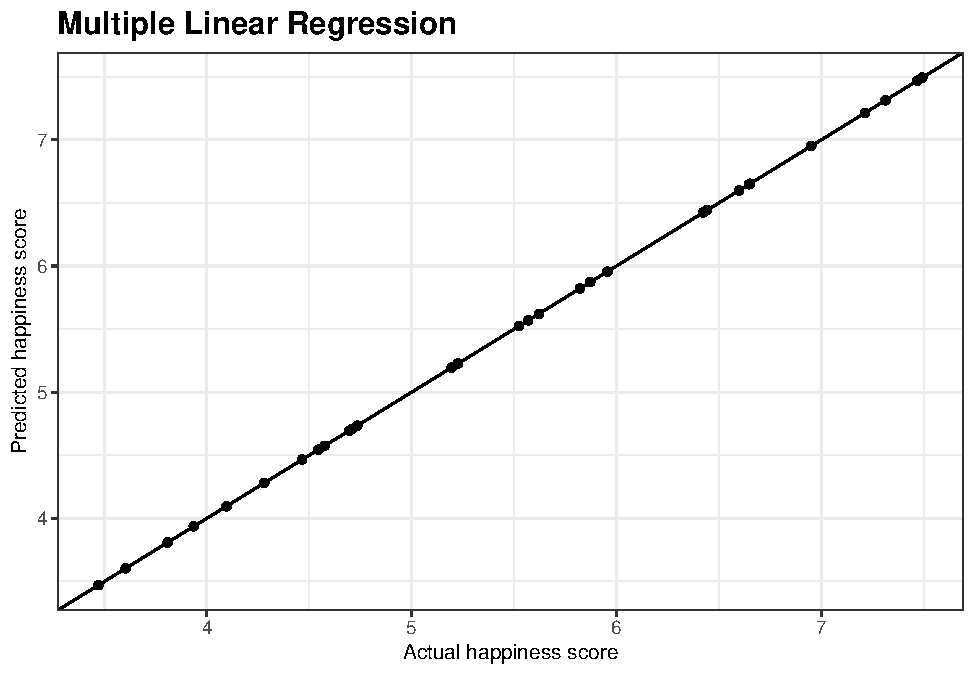
\includegraphics{Fer_files/figure-latex/unnamed-chunk-34-1.pdf}

As we expected, actual versus predicted plot shows the accuracy of our
model.

\textbf{SVR}

\begin{Shaded}
\begin{Highlighting}[]
\CommentTok{\# Fitting SVR to the dataset}
\FunctionTok{library}\NormalTok{(e1071)}
\NormalTok{regressor\_svr }\OtherTok{=} \FunctionTok{svm}\NormalTok{(}\AttributeTok{formula =}\NormalTok{ Happiness.Score }\SpecialCharTok{\textasciitilde{}}\NormalTok{ .,}
                \AttributeTok{data =}\NormalTok{ dataset,}
                \AttributeTok{type =} \StringTok{\textquotesingle{}eps{-}regression\textquotesingle{}}\NormalTok{,}
                \AttributeTok{kernel =} \StringTok{\textquotesingle{}radial\textquotesingle{}}\NormalTok{)}
\end{Highlighting}
\end{Shaded}

\begin{Shaded}
\begin{Highlighting}[]
\CommentTok{\# Predicting a new result}
\NormalTok{y\_pred\_svr }\OtherTok{=} \FunctionTok{predict}\NormalTok{(regressor\_svr,  }\AttributeTok{newdata =}\NormalTok{ test\_set)}

\NormalTok{Pred\_Actual\_svr }\OtherTok{\textless{}{-}} \FunctionTok{as.data.frame}\NormalTok{(}\FunctionTok{cbind}\NormalTok{(}\AttributeTok{Prediction =}\NormalTok{ y\_pred\_svr, }\AttributeTok{Actual =}\NormalTok{ test\_set}\SpecialCharTok{$}\NormalTok{Happiness.Score))}


\NormalTok{Pred\_Actual\_lm.versus.svr }\OtherTok{\textless{}{-}} \FunctionTok{cbind}\NormalTok{(}\AttributeTok{Prediction.lm =}\NormalTok{ y\_pred\_lm, }\AttributeTok{Prediction.svr =}\NormalTok{ y\_pred\_svr, }\AttributeTok{Actual =}\NormalTok{ test\_set}\SpecialCharTok{$}\NormalTok{Happiness.Score)}


\NormalTok{gg.svr }\OtherTok{\textless{}{-}} \FunctionTok{ggplot}\NormalTok{(Pred\_Actual\_svr, }\FunctionTok{aes}\NormalTok{(Actual, Prediction )) }\SpecialCharTok{+}
  \FunctionTok{geom\_point}\NormalTok{() }\SpecialCharTok{+} \FunctionTok{theme\_bw}\NormalTok{() }\SpecialCharTok{+} \FunctionTok{geom\_abline}\NormalTok{() }\SpecialCharTok{+}
  \FunctionTok{labs}\NormalTok{(}\AttributeTok{title =} \StringTok{"SVR"}\NormalTok{, }\AttributeTok{x =} \StringTok{"Actual happiness score"}\NormalTok{,}
       \AttributeTok{y =} \StringTok{"Predicted happiness score"}\NormalTok{) }\SpecialCharTok{+}
  \FunctionTok{theme}\NormalTok{(}\AttributeTok{plot.title =} \FunctionTok{element\_text}\NormalTok{(}\AttributeTok{family =} \StringTok{"Helvetica"}\NormalTok{, }\AttributeTok{face =} \StringTok{"bold"}\NormalTok{, }\AttributeTok{size =}\NormalTok{ (}\DecValTok{15}\NormalTok{)), }
        \AttributeTok{axis.title =} \FunctionTok{element\_text}\NormalTok{(}\AttributeTok{family =} \StringTok{"Helvetica"}\NormalTok{, }\AttributeTok{size =}\NormalTok{ (}\DecValTok{10}\NormalTok{)))}
\NormalTok{gg.svr}
\end{Highlighting}
\end{Shaded}

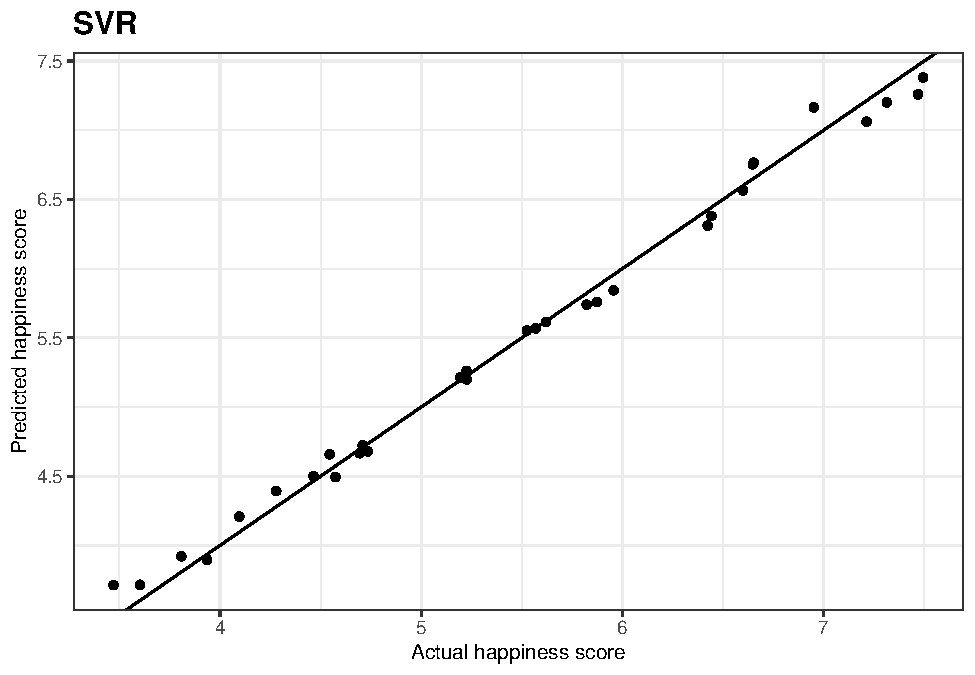
\includegraphics{Fer_files/figure-latex/unnamed-chunk-36-1.pdf}

Support Vector Regression predicted happiness scores with pretty high
accuracy.

\textbf{Decision Tree Regression}

\begin{Shaded}
\begin{Highlighting}[]
\CommentTok{\# Fitting Decision Tree Regression to the dataset}
\FunctionTok{library}\NormalTok{(rpart)}
\NormalTok{regressor\_dt }\OtherTok{=} \FunctionTok{rpart}\NormalTok{(}\AttributeTok{formula =}\NormalTok{ Happiness.Score }\SpecialCharTok{\textasciitilde{}}\NormalTok{ .,}
                  \AttributeTok{data =}\NormalTok{ dataset,}
                  \AttributeTok{control =} \FunctionTok{rpart.control}\NormalTok{(}\AttributeTok{minsplit =} \DecValTok{10}\NormalTok{))}
\end{Highlighting}
\end{Shaded}

\begin{Shaded}
\begin{Highlighting}[]
\CommentTok{\# Predicting a new result with Decision Tree Regression}
\NormalTok{y\_pred\_dt }\OtherTok{=} \FunctionTok{predict}\NormalTok{(regressor\_dt, }\AttributeTok{newdata =}\NormalTok{ test\_set)}

\NormalTok{Pred\_Actual\_dt }\OtherTok{\textless{}{-}} \FunctionTok{as.data.frame}\NormalTok{(}\FunctionTok{cbind}\NormalTok{(}\AttributeTok{Prediction =}\NormalTok{ y\_pred\_dt, }\AttributeTok{Actual =}\NormalTok{ test\_set}\SpecialCharTok{$}\NormalTok{Happiness.Score))}


\NormalTok{gg.dt }\OtherTok{\textless{}{-}} \FunctionTok{ggplot}\NormalTok{(Pred\_Actual\_dt, }\FunctionTok{aes}\NormalTok{(Actual, Prediction )) }\SpecialCharTok{+}
  \FunctionTok{geom\_point}\NormalTok{() }\SpecialCharTok{+} \FunctionTok{theme\_bw}\NormalTok{() }\SpecialCharTok{+} \FunctionTok{geom\_abline}\NormalTok{() }\SpecialCharTok{+}
  \FunctionTok{labs}\NormalTok{(}\AttributeTok{title =} \StringTok{"Decision Tree Regression"}\NormalTok{, }\AttributeTok{x =} \StringTok{"Actual happiness score"}\NormalTok{,}
       \AttributeTok{y =} \StringTok{"Predicted happiness score"}\NormalTok{) }\SpecialCharTok{+}
  \FunctionTok{theme}\NormalTok{(}\AttributeTok{plot.title =} \FunctionTok{element\_text}\NormalTok{(}\AttributeTok{family =} \StringTok{"Helvetica"}\NormalTok{, }\AttributeTok{face =} \StringTok{"bold"}\NormalTok{, }\AttributeTok{size =}\NormalTok{ (}\DecValTok{15}\NormalTok{)), }
        \AttributeTok{axis.title =} \FunctionTok{element\_text}\NormalTok{(}\AttributeTok{family =} \StringTok{"Helvetica"}\NormalTok{, }\AttributeTok{size =}\NormalTok{ (}\DecValTok{10}\NormalTok{)))}
\NormalTok{gg.dt}
\end{Highlighting}
\end{Shaded}

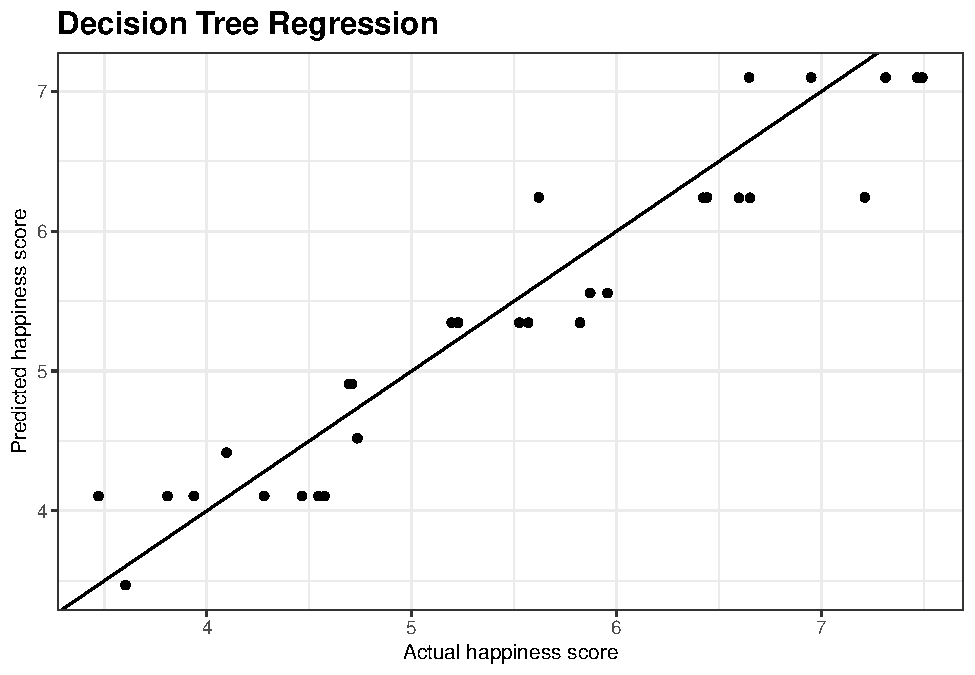
\includegraphics{Fer_files/figure-latex/unnamed-chunk-38-1.pdf}

It seems that Decision Tree Regression is not an excellent choice for
this dataset. Let's see the tree.

\begin{Shaded}
\begin{Highlighting}[]
\CommentTok{\# Plotting the tree}
\FunctionTok{library}\NormalTok{(rpart.plot)}
\FunctionTok{prp}\NormalTok{(regressor\_dt)}
\end{Highlighting}
\end{Shaded}

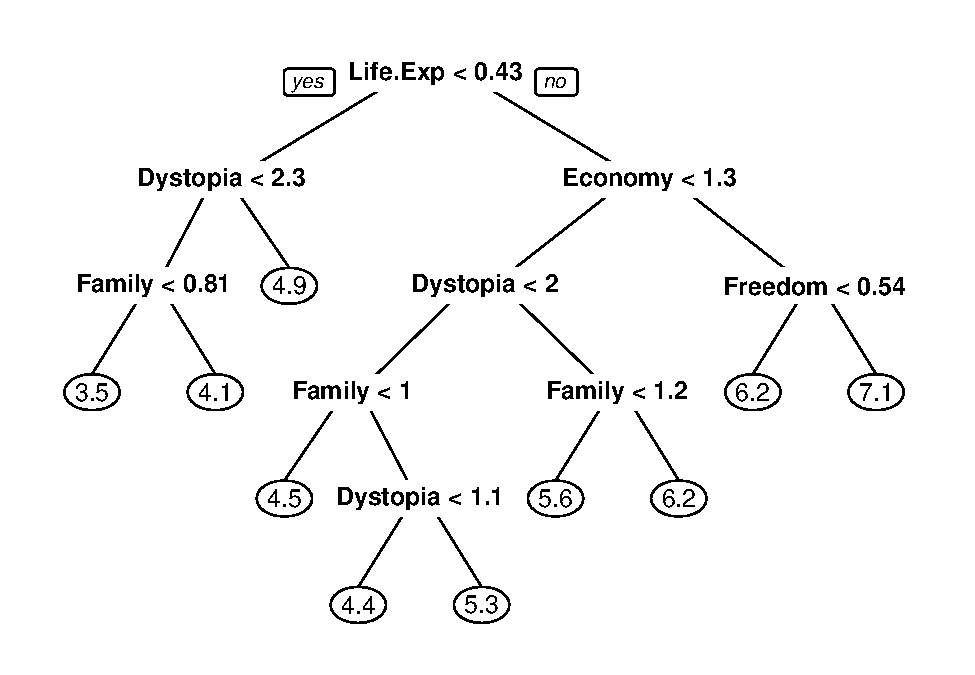
\includegraphics{Fer_files/figure-latex/unnamed-chunk-39-1.pdf}

\textbf{Random Forest Regression}

\begin{Shaded}
\begin{Highlighting}[]
\CommentTok{\# Fitting Random Forest Regression to the dataset}
\FunctionTok{library}\NormalTok{(randomForest)}
\FunctionTok{set.seed}\NormalTok{(}\DecValTok{1234}\NormalTok{)}
\NormalTok{regressor\_rf }\OtherTok{=} \FunctionTok{randomForest}\NormalTok{(}\AttributeTok{x =}\NormalTok{ dataset[}\SpecialCharTok{{-}}\DecValTok{1}\NormalTok{],}
                         \AttributeTok{y =}\NormalTok{ dataset}\SpecialCharTok{$}\NormalTok{Happiness.Score,}
                         \AttributeTok{ntree =} \DecValTok{500}\NormalTok{)}
\end{Highlighting}
\end{Shaded}

\begin{Shaded}
\begin{Highlighting}[]
\CommentTok{\# Predicting a new result with Random Forest Regression}
\NormalTok{y\_pred\_rf }\OtherTok{=} \FunctionTok{predict}\NormalTok{(regressor\_rf, }\AttributeTok{newdata =}\NormalTok{ test\_set)}

\NormalTok{Pred\_Actual\_rf }\OtherTok{\textless{}{-}} \FunctionTok{as.data.frame}\NormalTok{(}\FunctionTok{cbind}\NormalTok{(}\AttributeTok{Prediction =}\NormalTok{ y\_pred\_rf, }\AttributeTok{Actual =}\NormalTok{ test\_set}\SpecialCharTok{$}\NormalTok{Happiness.Score))}


\NormalTok{gg.rf }\OtherTok{\textless{}{-}} \FunctionTok{ggplot}\NormalTok{(Pred\_Actual\_rf, }\FunctionTok{aes}\NormalTok{(Actual, Prediction )) }\SpecialCharTok{+}
  \FunctionTok{geom\_point}\NormalTok{() }\SpecialCharTok{+} \FunctionTok{theme\_bw}\NormalTok{() }\SpecialCharTok{+} \FunctionTok{geom\_abline}\NormalTok{() }\SpecialCharTok{+}
  \FunctionTok{labs}\NormalTok{(}\AttributeTok{title =} \StringTok{"Random Forest Regression"}\NormalTok{, }\AttributeTok{x =} \StringTok{"Actual happiness score"}\NormalTok{,}
       \AttributeTok{y =} \StringTok{"Predicted happiness score"}\NormalTok{) }\SpecialCharTok{+}
  \FunctionTok{theme}\NormalTok{(}\AttributeTok{plot.title =} \FunctionTok{element\_text}\NormalTok{(}\AttributeTok{family =} \StringTok{"Helvetica"}\NormalTok{, }\AttributeTok{face =} \StringTok{"bold"}\NormalTok{, }\AttributeTok{size =}\NormalTok{ (}\DecValTok{15}\NormalTok{)), }
        \AttributeTok{axis.title =} \FunctionTok{element\_text}\NormalTok{(}\AttributeTok{family =} \StringTok{"Helvetica"}\NormalTok{, }\AttributeTok{size =}\NormalTok{ (}\DecValTok{10}\NormalTok{)))}
\NormalTok{gg.rf}
\end{Highlighting}
\end{Shaded}

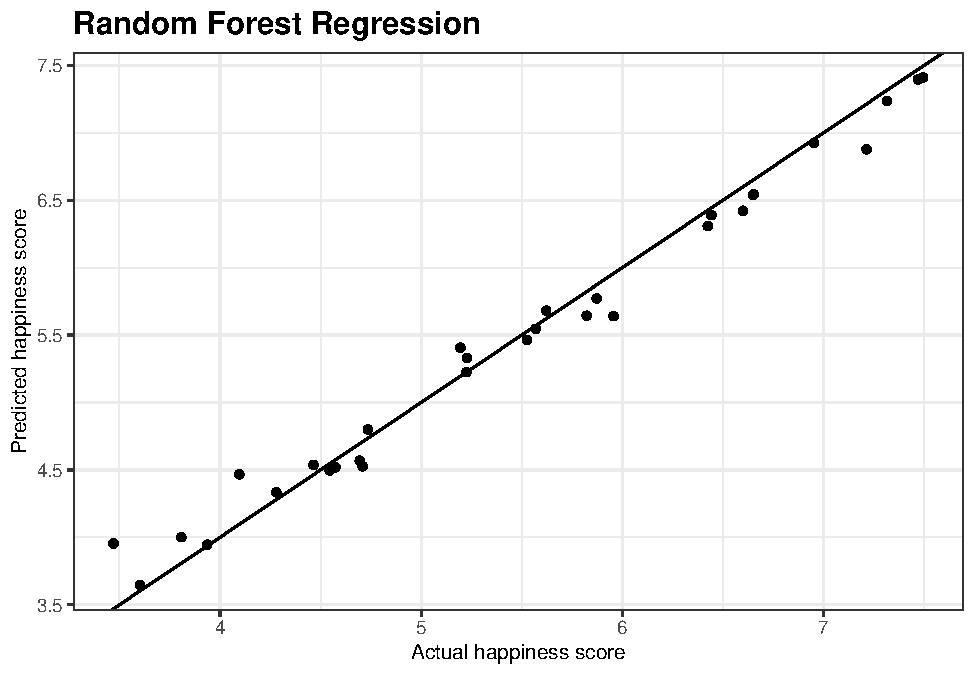
\includegraphics{Fer_files/figure-latex/unnamed-chunk-41-1.pdf}

Randon Forest regression is not as good as SVR regarding predicted
happiness scores but did a better job than Decision Tree.

\textbf{Neural Net}

\begin{Shaded}
\begin{Highlighting}[]
\CommentTok{\# Fitting Neural Net to the training set}
\FunctionTok{library}\NormalTok{(neuralnet)}

\NormalTok{nn }\OtherTok{\textless{}{-}} \FunctionTok{neuralnet}\NormalTok{(Happiness.Score }\SpecialCharTok{\textasciitilde{}}\NormalTok{ Economy }\SpecialCharTok{+}\NormalTok{ Family }\SpecialCharTok{+}\NormalTok{ Life.Expectancy }\SpecialCharTok{+}\NormalTok{ Freedom }\SpecialCharTok{+}\NormalTok{ Generosity }\SpecialCharTok{+}\NormalTok{ Trust }\SpecialCharTok{+}\NormalTok{ Dystopia.Residual,}
                \AttributeTok{data=}\NormalTok{training\_set,}\AttributeTok{hidden=}\DecValTok{10}\NormalTok{,}\AttributeTok{linear.output=}\ConstantTok{TRUE}\NormalTok{)}
\FunctionTok{plot}\NormalTok{(nn)}
\end{Highlighting}
\end{Shaded}

\begin{Shaded}
\begin{Highlighting}[]
\NormalTok{predicted.nn.values }\OtherTok{\textless{}{-}} \FunctionTok{compute}\NormalTok{(nn,test\_set[,}\DecValTok{2}\SpecialCharTok{:}\DecValTok{8}\NormalTok{])}

\NormalTok{Pred\_Actual\_nn }\OtherTok{\textless{}{-}} \FunctionTok{as.data.frame}\NormalTok{(}\FunctionTok{cbind}\NormalTok{(}\AttributeTok{Prediction =}\NormalTok{ predicted.nn.values}\SpecialCharTok{$}\NormalTok{net.result, }\AttributeTok{Actual =}\NormalTok{ test\_set}\SpecialCharTok{$}\NormalTok{Happiness.Score))}

\NormalTok{gg.nn }\OtherTok{\textless{}{-}} \FunctionTok{ggplot}\NormalTok{(Pred\_Actual\_nn, }\FunctionTok{aes}\NormalTok{(Actual, V1 )) }\SpecialCharTok{+}
  \FunctionTok{geom\_point}\NormalTok{() }\SpecialCharTok{+} \FunctionTok{theme\_bw}\NormalTok{() }\SpecialCharTok{+} \FunctionTok{geom\_abline}\NormalTok{() }\SpecialCharTok{+}
  \FunctionTok{labs}\NormalTok{(}\AttributeTok{title =} \StringTok{"Neural Net"}\NormalTok{, }\AttributeTok{x =} \StringTok{"Actual happiness score"}\NormalTok{,}
       \AttributeTok{y =} \StringTok{"Predicted happiness score"}\NormalTok{) }\SpecialCharTok{+}
  \FunctionTok{theme}\NormalTok{(}\AttributeTok{plot.title =} \FunctionTok{element\_text}\NormalTok{(}\AttributeTok{family =} \StringTok{"Helvetica"}\NormalTok{, }\AttributeTok{face =} \StringTok{"bold"}\NormalTok{, }\AttributeTok{size =}\NormalTok{ (}\DecValTok{15}\NormalTok{)), }
      \AttributeTok{axis.title =} \FunctionTok{element\_text}\NormalTok{(}\AttributeTok{family =} \StringTok{"Helvetica"}\NormalTok{, }\AttributeTok{size =}\NormalTok{ (}\DecValTok{10}\NormalTok{)))}
\NormalTok{gg.nn}
\end{Highlighting}
\end{Shaded}

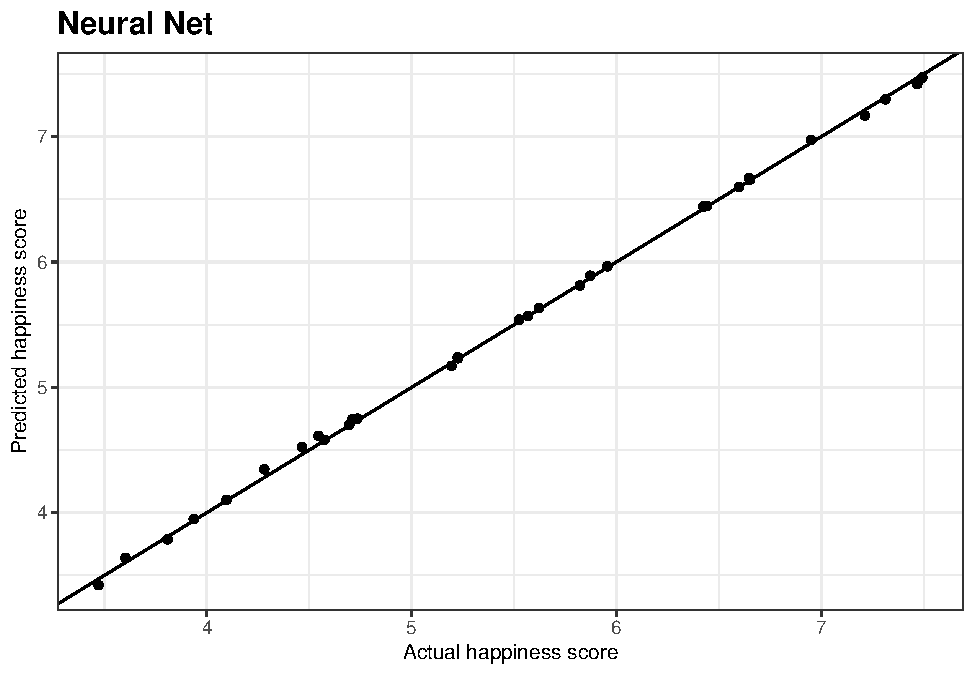
\includegraphics{Fer_files/figure-latex/unnamed-chunk-43-1.pdf}

Neural Net is the best predictor after Multiple Linear Regression. In
fact, this model predicted happiness scores with the accuracy close to
100 \%. Let's calculate the mean squared error for Multiple Linear
Regression and Neural Net model.

\begin{Shaded}
\begin{Highlighting}[]
\NormalTok{MSE.lm }\OtherTok{\textless{}{-}} \FunctionTok{sum}\NormalTok{((test\_set}\SpecialCharTok{$}\NormalTok{Happiness.Score }\SpecialCharTok{{-}}\NormalTok{ y\_pred\_lm)}\SpecialCharTok{\^{}}\DecValTok{2}\NormalTok{)}\SpecialCharTok{/}\FunctionTok{nrow}\NormalTok{(test\_set)}
\NormalTok{MSE.nn }\OtherTok{\textless{}{-}} \FunctionTok{sum}\NormalTok{((test\_set}\SpecialCharTok{$}\NormalTok{Happiness.Score }\SpecialCharTok{{-}}\NormalTok{ predicted.nn.values}\SpecialCharTok{$}\NormalTok{net.result)}\SpecialCharTok{\^{}}\DecValTok{2}\NormalTok{)}\SpecialCharTok{/}\FunctionTok{nrow}\NormalTok{(test\_set)}

\FunctionTok{print}\NormalTok{(}\FunctionTok{paste}\NormalTok{(}\StringTok{"Mean Squared Error (Multiple Linear Regression):"}\NormalTok{, MSE.lm))}
\end{Highlighting}
\end{Shaded}

\begin{verbatim}
## [1] "Mean Squared Error (Multiple Linear Regression): 9.12868493257418e-08"
\end{verbatim}

\begin{Shaded}
\begin{Highlighting}[]
\FunctionTok{print}\NormalTok{(}\FunctionTok{paste}\NormalTok{(}\StringTok{"Mean Squared Error (Neural Net):"}\NormalTok{, MSE.nn))}
\end{Highlighting}
\end{Shaded}

\begin{verbatim}
## [1] "Mean Squared Error (Neural Net): 0.000837343644496843"
\end{verbatim}

As we expected, mean squared error for Multiple Linear Regression is
smaller that Neural Net.

\textbf{Real versus predicted for different machine learning
algorithms}\\
Let's see one more time the result of our predictors to see their
accuracy visually.

\begin{Shaded}
\begin{Highlighting}[]
\FunctionTok{ggarrange}\NormalTok{(gg.lm, gg.svr, gg.dt, gg.rf, gg.nn, }\AttributeTok{ncol =} \DecValTok{2}\NormalTok{, }\AttributeTok{nrow =} \DecValTok{3}\NormalTok{)}
\end{Highlighting}
\end{Shaded}

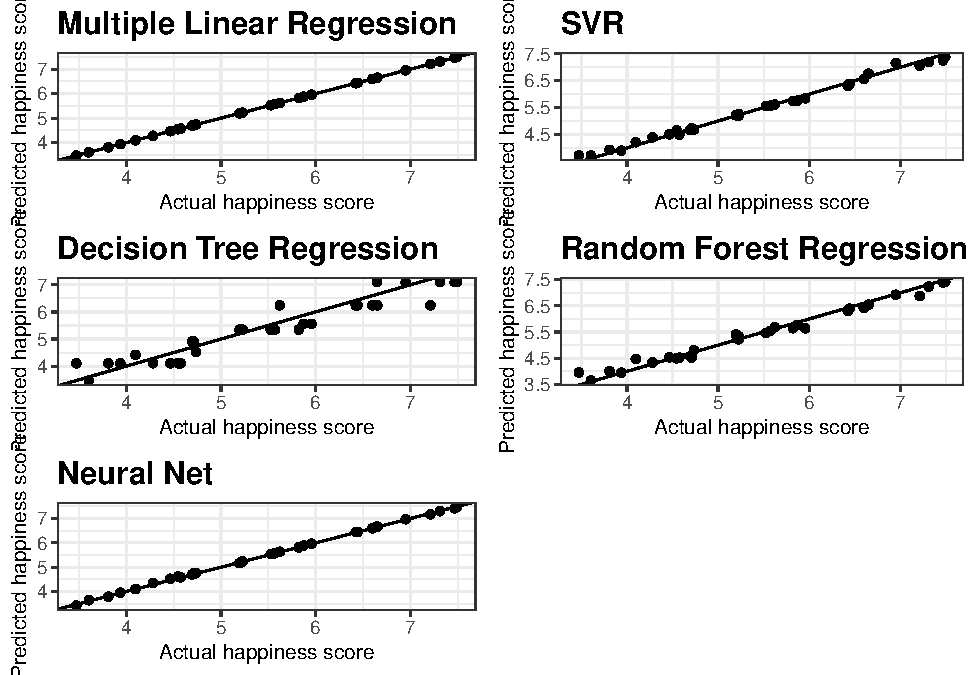
\includegraphics{Fer_files/figure-latex/unnamed-chunk-45-1.pdf}

Multiple Linear Regression and neural net did the best job and predicted
approximately the same. SVR and Random Forest stood in the second place
regarding accuracy in prediction. And finally, Decision Tree was the
worst algorithm to predict happiness scores.

\end{document}
